\chapter{Sociolinguistic variation in Jamaican English}\label{ch:3}
\section{Level of education}\label{sec:3.1}

As noted in \chapref{ch:1}, DeCamp’s original characterization of the \isi{acrolect} was the speech of  “the well-educated urban professional” (\citeyear[82]{DeCamp1961}).  And in any reading of the literature on the Caribbean, education is the single most important social factor used to locate the speaker of the \isi{standard variety} of English.\footnote{Other factors like social class (typically indexed by occupation and income), urban provenance and, to a lesser extent, \isi{race}\slash \isi{skin colour} have also been used (see the discussion in \sectref{sec:1.4} of this book).  However, with the possible exception of \isi{race}\slash \isi{skin colour}, factors like class, residence and occupation are themselves inextricably linked to the speaker’s level of education.}  This is not peculiar to the Caribbean, however, as educatedness is important for locating the standard speaker elsewhere.  \citet[118]{Trudgill1999} can be used as an example:

\begin{quote}
...it is the variety associated with the education system in all the English-speaking countries of the world, and is therefore the variety spoken by those who are often referred to as ``educated people''. 
\end{quote}

This, of course, implies that the perception of a speaker as “educated” can influence the way we evaluate their language use as standard, possibly as much as the structures used in speech \citep{ThakerarGilesCheshire1982}.

As stated earlier, the \textit{Revised primary curriculum} 1999, published by the \isi{Ministry of Education} in Jamaica, conceives of a locally legitimised target variety for the school system, \isi{SJE}.

Historically, English has been the one compulsory exam taken in Jamaica, and the data indicate that, on average, roughly 40\% of CXC candidates achieve grades acceptable for tertiary education (\citealt[222]{Miller1989}).  A similar percentage of students, according to the Ministry, passed in 2000:\footnote{These results are controversial as they reflect the percentage of students allowed to sit the exam, not students eligible to sit.  When students eligible to sit are analysed, then the percentage of students achieving the appropriate English Language grade is halved.  For example, in 2003, by reason of pre-selection, 16,000 students were not allowed to take the CXC exam in English, an average exclusion rate of about 50 percent (\textit{The Daily Gleaner}, November 21, 2003).}%Moved Footnote because this was the only way to avoid a bad pagebreak.

\begin{quote}
	In English Language, the passes moved from the 41.2 per cent in 1999 to 47.9 this year [2000]. Grades 1, 2 and 3 are the acceptable grades for entry into tertiary institutions (\textit{The Daily Gleaner}, September 2, 2000).
\end{quote}

The \isi{SJE} described by the \citet[17]{Curriculum1999} has only a handful of phonological prescriptions for the teacher\slash student:

\begin{itemize}
\item 
distinguish between false homophones in JC and \isi{SJE} e.g. \textit{at}\slash\textit{hot}, \textit{an}\slash\textit{on}, \textit{doze}\slash\textit{those}
\item 
clarify JC\slash \isi{SJE} confusion of words such as \textit{file}\slash\textit{foil}
\end{itemize}

Interestingly, in light of the discussion in the previous chapter, these pinpoint for the teacher and the student – phonemic /h/ usage, control of the [\textbf{ɔ}] vowel and TH stopping.  This might suggest some predictable outcomes in any correlation of language use and education in this study.  We might, for example, expect a greater degree of uniformity in the use of the variants [h], [\textbf{ɔ}] and [θ/ð], focussed by the prescriptions of the school system.  Additionally, the informants with higher education and more prolonged exposure to the school system might produce fewer non-stan\-dard variants of these variables.    

Within \isi{JAMPRO} itself, education was the most important of the criteria mentioned for employment and success at the agency.  Of the 104 informants in this study, 77 (74\%) specifically said that having at least a (University) degree was essential, and they suggested the following reasons why:

\begin{itemize}
\item\relax [it gives you] an ability to see the bigger picture and think a little differently (F50)
\item if you’re well educated and everything your social class tends to be middle class (F56)
\item it equips you to have a good command of the English language (F7)
\item it gives you an edge (F21)
\item it impresses (F46).
\end{itemize}

One consequence of this agency policy is that \isi{JAMPRO} staff is highly educated relative to the wider society \citep[15:22]{STATIN1991}.\footnote{The category “post-secondary” refers to those employees who have completed high school and gone on to do courses, diplomas or certificates at some institution; “tertiary” then refers specifically to a university degree.  The Jamaica data does not add up to 100\%, as I have not included the uneducated (i.e. unschooled) in the table.}

\begin{table}
\begin{tabular}{lSS}
\lsptoprule
 & \multicolumn{1}{c}{\isi{JAMPRO} (All) (\%)} & \multicolumn{1}{c}{Jamaica (\%)}\\\midrule
Primary        & 4 & 50\\
Secondary      & 10 & 29.4 \\
Post-Secondary & 42 & 18.6\\
Tertiary       & 21 & 1.3\\
Postgraduate   & 23 & 0.7\\
\lspbottomrule
\end{tabular}
\caption{JAMPRO and Jamaican educational attainment compared}
\label{tab:3.1}
\end{table}

Most of the staff has post-secondary as minimum level of education, with close to half of the total sample being university educated.  All but the primary level informants have therefore achieved Grades 1, 2 or 3 or equivalent in English examinations at least at the CXC or GCE ``O'' level standard.  Those with a university degree, will also have completed tertiary level English language courses such as UWI’s English for Academic Purposes. 

Of those informants whose speech was recorded, the distribution is as in \tabref{tab:3.2}.\footnote{One informant did not give a response and therefore the total for \isi{JAMPRO} adds up to 103.}

\begin{table}
\begin{tabular}{lr@{ }Sr@{ }S} 
\lsptoprule
& \multicolumn{2}{c}{\isi{JAMPRO} (All) (\%)} & \multicolumn{2}{c}{Jamaica (\%)}\\\midrule
Primary        & 4  & (3.9\%)  & 4  & (4.9\%)\\
Secondary      & 10 & (9.7\%)  & 9  & (11.1\%)\\
Post-Secondary & 43 & (41.7\%) & 36 & (44.4\%)\\
Tertiary       & 22 & (21.4\%) & 16 & (19.8\%)\\
Postgraduate   & 24 & (23.3\%) & 16 & (19.8\%)\\
\lspbottomrule
\end{tabular}
\caption{JAMPRO educational attainment and informants compared\label{tab:3.2}}
\end{table}

It should be mentioned that for many members of staff, the importance placed on “having a degree” was a contentious issue.  Two attitudes were observed.  The first was a resentment that \isi{JAMPRO} placed more stock in the “piece of paper” than it did on actual performance.  A few informants expressed the perception that the requirements for promotion, in particular, stressed further education over an ability to do the job.  This was a decidedly minority view from 5 informants.  A more common feeling was that \isi{JAMPRO} favoured candidates with foreign degrees, earned outside of the Caribbean.  Twenty-three (23) informants specifically said that having a foreign degree meant a greater chance of being hired and better prospects in the company.  Of the 46 informants with tertiary level qualifications, 12 (26\%) had degrees from either the USA or the EU and, not surprisingly, neither they nor \isi{senior management} shared this perception.

Level of education will of course be an intervening variable in a number of the other social categories discussed in this study, such as status in the company and frontline position.  In this section, however, I am only interested in any correlations that can be made with education alone, and where it is relevant in subsequent sections it will be discussed there.  The educational categories have been collapsed into “primary”, “secondary+” and “tertiary+”, for in many correlations tokens were not enough to support a more nuanced stratification.  The statistical analyses that follow \textit{exclude} primary educated speakers; by inspection their patterns of use are very different and, when included in the chi-squared tests, they tend to distort the results.  Moreover, as there were only four such informants in the agency, sufficient data could not be collected for many variables.

  In the tables below the data for the 4 primary educated informants will be displayed so that their patterns can be compared to that of the other informants.\footnote{All correlations were done using a chi-squared test of association.  My interest here was not to weigh the relative influence of several factors on the production of informants or groups of informants.  Indeed, the ultimate purpose of the study is to describe the speech of a particular subset of the \isi{JAMPRO} sample, who constitute a specific, select set of employees (see \chapref{ch:4}).  For that, and because of the type of data collected (frequencies and not scores), I used a non-parametric statistical procedure.  I accept as statistically significant any association that yields a probability value of less than 5\% (<.05).  However, I also comment on data that produces results close to that value.}

\subsection{{Group} {A} {variables} {and} {education}}%3.1.1n

\begin{table}
\begin{tabular}{lr*{2}{r@{ }r}}
\lsptoprule
       &    n  &   \multicolumn{2}{c}{h-drop}   & \multicolumn{2}{c}{h} \\
\midrule
Primary     &  4  & 18 & (37\%) & 31 & (63\%)\\
Secondary+ &  45 & 127 & (17\%) & 636  & (83\%)\\
Tertiary+  &  32 & 39 & (5\%) & 729 & (95\%)\\
\lspbottomrule
\end{tabular}
\caption{h-drop by education level (p < .001, χ\textsuperscript{2} = 59.72)}
\label{tab:3.3}
\end{table}

  There is a clear correlation between frequency of \isi{h-drop} and level of education, with less of the feature used as the level of education rises.  University graduates almost never \isi{h-drop}, though all informants generally produce relatively low frequencies of the feature.  Of the four primary informants, one (M40) never dropped [h] (see \tabref{tab:4.16} on page~\pageref{tab:4.16} on \isi{frontline staff}).  The few attestations of hypercorrect use, – that is, “incorrectly” adding [h] – were most typical in the “secondary+” cohort (6 of the 9 informants who produced it), along with one “tertiary+” informant (M101), and two primary educated speakers.  Seemingly, there were no h-less lects in my sample, though one informant (M88) produced [h] only once in his discourse. 


\begin{table}
\begin{tabular}{l*{4}{r@{ }S}}
\lsptoprule
{Word Initial}  &  \multicolumn{2}{c}{d} &   \multicolumn{2}{c}{ð}  &  \multicolumn{2}{c}{t}  &  \multicolumn{2}{c}{θ}\\\midrule
Primary             & 111  & (92.5\%)  &     9 & (7.5\%)  & 13 & (59.0\%)  &     9 & (41.0\%)\\
Secondary+          & 1205 & (56.0\%)  &   940 & (44.0\%) & 78 & (18.4\%)  &   345 & (81.6\%)\\
Tertiary+           & 920  & (49.0\%)  &   965 & (51.0\%) & 25 & (7.0\%)   &   341 & (93.0\%)\\\cmidrule(lr){2-5}\cmidrule(lr){6-9}
& \multicolumn{4}{c}{(p < .001, χ\textsuperscript{2} = 21.86)} & \multicolumn{4}{c}{(p < .001, χ\textsuperscript{2} = 23.24)}\\\midrule
{Word Middle}  &  \multicolumn{2}{c}{d} &   \multicolumn{2}{c}{ð}  &  \multicolumn{2}{c}{t}  &  \multicolumn{2}{c}{θ}\\\midrule
Primary              & 10 & (71.4\%)   &    4 & (28.6\%) &  2  & (100.0\%)  &     0 & \\
Secondary+           & 36 & (23.0\%)   &  120 & (77.0\%) & 13  & (18.6\%)   &    57 & (81.4\%)\\
Tertiary+            & 27 & (21.0\%)   &  100 & (79.0\%) &  7  & (15.6\%)   &    38 & (84.4\%)\\\cmidrule(lr){2-5}\cmidrule(lr){6-9}
       & \multicolumn{4}{c}{(p > .70, χ\textsuperscript{2} = 0.117)} &    \multicolumn{4}{c}{(p > .50, χ\textsuperscript{2} = 0.17)}\\\midrule
{Word Final}  &  \multicolumn{2}{c}{d} &   \multicolumn{2}{c}{ð}  &  \multicolumn{2}{c}{t}  &  \multicolumn{2}{c}{θ}\\\midrule
Primary              & 6  & (100.0\%)     &   0  &          & 0  &        &    0  &       \\
Secondary+           & 12 & (20.0\%)      &   48 & (80.0\%) & 11 & (29.0\%) &   27 & (71.0\%)\\
Tertiary+            & 15 & (27.0\%)      &   40 & (73.0\%) & 8  & (18.0\%) &   36 & (82.0\%)\\\cmidrule(lr){2-5}\cmidrule(lr){6-9}
& \multicolumn{4}{c}{(p > .30, χ\textsuperscript{2} = 0.8)}  &     \multicolumn{4}{c}{(p > .20, χ\textsuperscript{2} = 1.27)}\\
\lspbottomrule
\end{tabular}
\caption{TH stopping by education level}
\label{tab:3.4}
\end{table}

  Word finally and in middle position there is no statistically significant difference between “secondary+” and “tertiary+” informants.  Both sets of speakers have similarly low levels of TH stopping, whether voiced or voiceless, though the data set per speaker is small and generalizations must be cautiously made.  Word initially, the more educated the speaker the lower the incidence of TH stopping, particularly when voiceless.  Only one informant (M14) produced a high proportion of the voiceless stop variant.  He alone accounted for 7 of the 25 tokens of [t], suggesting that for most speakers in this group a more accurate characterization would be absence of voiceless TH stopping.  Importantly, tertiary+ informants who almost never use the voiceless stop variant, have close to half of their productions of the voiced variable as stops.  While we can say that tertiary+ educated speakers, who almost never vary [t {\textasciitilde} θ], produce much less of the \isi{Creole} form, we cannot say that their speech is characterized by more consistent use of the \isi{PJS} form [ð] in this case.     

\begin{table}

\begin{tabular}{l*{3}{r@{ }r}}
\lsptoprule
   &   \multicolumn{2}{c}{nat} & \multicolumn{2}{c}{nʌt}  & \multicolumn{2}{c}{nɔt}\\
\midrule
Primary    & 23  & (46\%) & 10  & (20\%) & 17  & (34\%)\\
Secondary+ & 263 & (25\%) & 184 & (17\%) & 610 & (58\%)\\
Tertiary+  & 96  & (12\%) & 127 & (16\%) & 573 & (72\%)\\
\lspbottomrule
\end{tabular}
\caption{The low back vowel and variants by education level             }
\label{tab:3.5}
\end{table}

In productions of \textit{not} type words, primary educated informants show a great deal of variation in their use of the \isi{low back vowel} variants – with [a] used most frequently – though it cannot be said that this use is focussed around the \isi{Creole} variant as more than half their attestations of the vowel are not the JC variant.  At the other educational levels, what distinguishes the groups is a greater frequency of use of the [ɔ] as level of education increases, and less use of the [a] (p\,<\,.001, χ\textsuperscript{2}\,=\,53.5).  The more central vowel [ʌ] is produced by all levels of informants at a similarly low rate. 

\begin{table}
\begin{tabular}{l*{4}{r@{ }r}}
\lsptoprule
    &       \multicolumn{2}{c}{uo}      &    \multicolumn{2}{c}{o}  & \multicolumn{2}{c}{ie}   &   \multicolumn{2}{c}{e}\\
\midrule
Primary     & 3  & (5.6\%)  &     51  & (94.4\%) & 11  & (27\%)   &      30 & (73\%)\\
Secondary+ & 89 & (9.0\%)    &     918 & (91.0\%)   & 174 & (16\%)   &     883 & (84\%)   \\
Tertiary+  & 37 & (6.0\%)    &     545 & (94.0\%)   & 76  & (11\%)   &     623 & (89\%)\\\cmidrule(lr){2-5}\cmidrule(lr){6-9}
   & \multicolumn{4}{c}{(p < .10, χ\textsuperscript{2} = 3.08)}  & \multicolumn{4}{c}{(p < .001, χ\textsuperscript{2} = 15.75)}\\
\lspbottomrule
\end{tabular}
\caption{Mid-vowels by education level}
\label{tab:3.6}
\end{table}

The statistical difference between speakers when it comes to the \isi{back diphthong} is below the critical level.  The tertiary educated do not use significantly fewer diphthongs than the secondary educated; and importantly, the primary educated informants also follow the general pattern of these speakers and more consistently use the monophthong.  In this formal context all speakers produced few [uo], though as discussed earlier, in Beckford-Wassink’s study, the pattern in informal speech is somewhat different.  It is use of the front [ie] that distinguishes speakers from the various levels of education, and as with initial voiceless TH stopping, \isi{h-drop} and the \isi{low vowel} [a], the higher the level of education the lower the incidence of the \isi{Creole} variant and the more the [e] is used.  However, it appears that not all \isi{Creole} features are evaluated in the same way.  Speakers generally are more likely to say [fies] than they are to say [guot]; and it is the more frequently used \isi{Creole} form that does distinguish educational groups at \isi{JAMPRO}.  If the [ie] is in wider use (see the previous section) then it may be more likely that judgements of social place will be linked to that variant, given a general avoidance of [uo] in the data.  This avoidance demonstrates a consensus across all educational groups here that [o] is the \isi{JE} form.  Contestation about what is \isi{JE} takes place with [e {\textasciitilde} ie], with education one factor determining frequency of use.  It is also just as likely that use of [uo] may index some other social difference, as in Beckford-Wassink’s (\citeyear[155]{BeckfordWassink2001}) study which showed a link to \isi{gender}.    

\begin{table}
\begin{tabular}{l *{5}{r@{ }r}}
\lsptoprule
&  \multicolumn{6}{c}{\textit{poor}  type words} &  \multicolumn{4}{c}{\textit{beer} type words}\\\cmidrule(lr){2-7}\cmidrule(lr){8-11}
&   \multicolumn{2}{c}{[ɔ]}  &  \multicolumn{2}{c}{[u\textsuperscript{o}]}  &  \multicolumn{2}{c}{[o]}  & \multicolumn{2}{c}{[i\textsuperscript{e}r]} & \multicolumn{2}{c}{[er]}\\
\midrule
Primary     & 6  & (40\%)   &          5 & (33\%) &         4 & (27\%) & 17  & (81\%) &     4 & (19\%)\\
Secondary+ & 246 & (77\%)   &         47 & (15\%) &        26 & (8\%)  & 241 & (51\%) &   234 & (49\%)\\
Tertiary+  & 192 & (70\%)   &         62 & (23\%) &        20 & (7\%)  & 222 & (40\%) &   332 & (60\%)\\\lspbottomrule
\end{tabular}
\caption{Pre-rhotic mid-vowels by education level}
\label{tab:3.7}
\end{table}

Higher education was correlated with fewer front diphthongs overall, and in pre-rhotic environments we find a similar pattern (p < .001, χ\textsuperscript{2} = 11.71).  However, the incidence of diphthongization is noticeably higher in \textit{beer} type words, with educated speakers varying almost freely between the two variants.  In \textit{poor} type words, educated speakers overwhelmingly select the [ɔr] variant and therefore have fairly low frequencies of dipthongization (p < .02, χ\textsuperscript{2} = 5.92).  However, those with tertiary+ education produce more of the diphthong than the secondary educated.  Higher education then does not necessarily disfavour use of the [u\textsuperscript{o}] variant, though we can identify which of the three is the \isi{JE} variant.  The secondary educated, in particular, are more likely than any other group to use the [ɔr] variant, perhaps approximating more to a prestige pattern that, from the data, seems to be use of the /ɔ/ rather than /o/.  Arguably, the stigma attached to using [uo], which speakers tend to avoid, as well as the prestige attached to the [ɔ] vowel in \isi{JE}, have reinforced the selection of the [ɔr] variant. 

\begin{table}
\begin{tabular}{l*{4}{r@{ }r}}
\lsptoprule
& \multicolumn{2}{c}{kja} & \multicolumn{2}{c}{k\textsuperscript{h}a} & \multicolumn{2}{c}{kja:} & \multicolumn{2}{c}{k\textsuperscript{h}a:}\\
\midrule
Primary & 5      & (50\%) &    5 & (50\%)      & 2  & (100\%)    &      0& \\
Secondary+ & 65 & (61\%) &   41 & (39\%)      & 13 & (28\%)     &      34 &(72\%)\\
Tertiary+ & 46  & (52\%) &   43 & (48\%)      & 4  & (9\%)      &      41 &(91\%)\\\cmidrule(lr){2-5}\cmidrule(lr){6-9}
   & \multicolumn{4}{c}{(p > .30, χ\textsuperscript{2} = 1.8)}        &        \multicolumn{4}{c}{(p < .05, χ\textsuperscript{2} = 5.36)}\\
\lspbottomrule
\end{tabular}
\caption{Word initial velar stops and variants by education level}
\label{tab:3.8}
\end{table}

The data set for this feature is small, at best 2 to 3 tokens per speaker recorded.  The discussion of these results is done with a full awareness of the problems of generalizing from such a small sampling.  The creation of word-lists to test informants, however, would not have been useful here to add to the data set.  Word-lists do not reflect the way people normally use or hear spoken language, even in formal contexts.  Moreover, they test what the informant perceives to be, for example, the standard form when it is isolated and made the focus of attention.  This does not necessarily reveal how the form is used when it is just one of a number of variables that the speaker uses\slash varies when producing discourse.    

The relatively high incidence of [kja] in the speakers with higher education is in sharp contrast to the incidence of [kja\textbf{:}], in particular for university graduates.  It is the production of the latter feature that distinguishes the two groups statistically.  Indeed, it is possible that the secondary educated pattern, with 61\% use of [kj] before the short [a], may reflect the type of \isi{quantitative hypercorrection} typically described for the LMC \citep[254]{Labov1980}.  This suggests either that [kja] is not perceived by speakers as \isi{Creole}, or that it is a feature that is found across the continuum, even in acrolectal speech (see \sectref{sec:3.4} on \isi{age}).  If so, in a linguistic culture in which perceptions are binary, then this feature cannot be regarded as \isi{Creole}, even though it occurs in JC.  When the tertiary educated are analysed in terms of  presence\slash absence of features, the following obtains.  In all cases the speakers had the opportunity to produce a particular variant.  

\begin{table}
\begin{tabular}{lcrrr}
\lsptoprule
        &                   &  \multicolumn{3}{c}{Variant}\\\cmidrule(lr){3-5}
Feature &  Informants taped &  \multicolumn{1}{c}{Never use} &  \multicolumn{2}{c}{Always use}\\\midrule
/h/ & 32 & 0 &\shadecell 17  &\shadecell (53\%)\\
{Initial [ð]} & 32 & 0 & 0\\
Initial [θ] & 32 & 0 &\shadecell 19  &\shadecell (59\%)\\
{[ɔ}] {\textit{not}} & 32 & 0 & 0\\
{[o] \textit{boat}} & 32 & 0 & 15  & (47\%)\\
{[e] \textit{face}} & 32 & 0 & 15  & (47\%)\\
{[ɔr] \textit{poor}} & 31 & 0 & 11  & (35\%)\\
{[ber] \textit{beer}} & 32 & 0 & 1  & (3\%)\\
{[k\textsuperscript{h}a]}  & 27 & 3 & 7  & (26\%)\\
{[k\textsuperscript{h}a:]} & 20 & 2 &  17 \shadecell  &  \shadecell (85\%)\\
\lspbottomrule
\end{tabular}
\caption{Group A variables and distribution in the highly educated (“Tertiary+” speakers)}
\label{tab:3.9}
\end{table}

  For the “tertiary+” speakers, [kja\textbf{:}], voiceless TH stopping and \isi{h-drop} are the three features that most do not produce in \isi{formal speech}.  To a lesser extent, diphthongs (except the pre-rhotic  [ie]) are also not an aspect of many informants’ texts.  But voiced TH stopping, [kja] and [nat] all occur in spoken \isi{JE}, though the data above suggest that in tertiary educated speakers the latter is infrequent in the individual’s speech even as it is a universally present variant.  

Notably, the pattern for primary educated speakers is clearly different (with a caveat about high percentages in a small sample).  Only h-dropping and [uo] were absent from the speech of anyone with primary education.  Interestingly, informant F96 produced no [uo] in her recording (for 15 instances of the variable), but produced [ie] for 6 of 13 instances of that variable (46\%).  

\subsection{{Group} {B} {variables} {and} {education}}%3.1.2n

\begin{table} 
\begin{tabular}{l*{3}{r@{ }S}}
\lsptoprule
& \multicolumn{2}{c}{butt[a]} & \multicolumn{2}{c}{butt[ʌ]} & \multicolumn{2}{c}{butt[ʌr]}  \\
\midrule
Primary    & 38   &(76.0\%) & 12 & (24.0\%) & 0 & \\
Secondary+ & 150  &(22.0\%) & 473& (69.0\%) & 60& (9.0\%)\\
Tertiary+  & 48   &(8.5\%) & 463 &(81.5\%) & 57 &(10.0\%)\\
\lspbottomrule
\end{tabular}
\caption{\textit{-er} word ending and variants by education level\label{tab:3.10}}
\end{table}

The suggestion made earlier in this section, that it is possibly only in the features perceived to be along the \isi{Creole}\slash English dimension that level of education is indexed, can be examined in relation to this set of variables.  Here, variation is not only between \isi{Creole}\slash English options but also includes alternants of \isi{JE} as well, though in many cases the phonetic options themselves can be explained in terms of avoiding certain \isi{Creole} forms (notably [a {\textasciitilde} ɔ] and affricates).  The data in \tabref{tab:3.10} show that production of the \isi{JE} \textit{butt}[ʌr] form is not what distinguishes the tertiary from the secondary educated; rather it is use of less [a] (the stereotypically \isi{Creole} variant) and more [ʌ] (p < .001, χ\textsuperscript{2} = 42.38).  This would seem to confirm the importance of the \isi{Creole}\slash English relationship in defining “good” or standard English in Jamaica, as reflected in the speech of the most educated.  Retroflexion of the word ending does not distinguish groups with higher education.     

\tabref{tab:3.11} below further illustrates the effect of \isi{Creole} avoidance strategies on speakers’ productions, but also lends support to the earlier comment that \isi{MSE} norms are not necessarily the only target of speakers either.    

\begin{table}
\begin{tabular}{l*{4}{r@{ }S}}
\lsptoprule
& \multicolumn{2}{c}{educa\textbf{[ʃan]}} & \multicolumn{2}{c}{educa\textbf{[ʃʌn]}} & \multicolumn{2}{c}{educa\textbf{[ʃɔn]}}  & \multicolumn{2}{c}{educa\textbf{[ʃǝn]}}\\
\midrule
Primary    & 11  & (85.0\%) & 2   & (15.0\%) & 0  &      & 0\\
Secondary+ & 102 & (30.0\%) & 171 & (50.0\%) & 39 & (11.0\%) & 31 & (9.0\%)\\
Tertiary+  & 31  & (9.0\%)  & 201 & (59.0\%) & 76 & (22.0\%) & 34 & (10.0\%)\\
\lspbottomrule
\end{tabular}
\caption{\textit{-tion} word ending and variants by education level}
\label{tab:3.11}
\end{table}

The frequency of use of the schwa is similar for the two higher education levels.  What accounts for the value of the χ\textsuperscript{2} is the difference in the use of [ʃan] and [ʃɔn] (p < .001, χ\textsuperscript{2} = 52.23).  Tertiary educated speakers use less of the \isi{Creole} variant, and more of the \isi{JE} alternant [ʃɔn].  Educatedness, arguably, is more clearly indexed by use of the locally evolved variant, not the \isi{MSE} schwa.  

  Interestingly, if the 7 informants with foreign degrees are isolated for discussion, their patterns of variation are, by inspection, different from the locally educated (see \tabref{tab:3.12}).

\begin{table}
\begin{tabular}{l*{4}{r@{ }S}}
\lsptoprule
& \multicolumn{2}{c}{educa\textbf{[ʃan]}} & \multicolumn{2}{c}{educa\textbf{[ʃʌn]}} & \multicolumn{2}{c}{educa\textbf{[ʃɔn]}}  & \multicolumn{2}{c}{educa\textbf{[ʃǝn]}}\\
\midrule
Foreign      &          3 & (4.0\%)     &  48 & (68.0\%)   &    11 & (15.0\%) & 9  & (13.0\%)\\
Local        &         28 & (10.25\%)   & 153 & (56.5\%)   &    65 & (24.0\%) & 25 & (9.25\%)\\\midrule
 & \multicolumn{2}{c}{butt[a]} & \multicolumn{2}{c}{butt[ʌ]} & \multicolumn{2}{c}{butt[ʌr]} &  & \\\midrule
Foreign       &        4  & (4.0\%)   &        87 & (83.0\%)  &      14 & (13.0\%)            &  & \\
Local         &        44 & (9.5\%)   &       376 & (81.0\%)  &      43 & (9.0\%)             &  & \\\lspbottomrule
\end{tabular}
\caption{Articulation of word endings by place of education}
\label{tab:3.12}
\end{table}

For these variables, the variation evident in the foreign educated informants is phonetically more akin to \isi{MSE}.  In the first table, there is a marginally greater frequency of schwa; the locally educated produce more [ʃɔn] and [ʃan] (p > .10, χ\textsuperscript{2} = 5.93).  And in the second table, “locals” produce fewer retroflex endings, and more [a], than those with overseas education (p < .10, χ\textsuperscript{2} = 4.9).  Among informants whose education has been entirely in Jamaica we find use of the \isi{Creole} variant and use of the local \isi{JE} variant(s) to be the main areas of difference between them.  Higher education in Jamaica then cannot necessarily be correlated with an increased use of the \isi{metropolitan norm}, but, as the data here would suggest and as would be expected, such norms are more likely in those who have been exposed to them.  

\begin{table}
\begin{tabular}{l *{4}{r@{ }S}}
\lsptoprule
   &   \multicolumn{2}{c}{dj} & \multicolumn{2}{c}{ʤ}  &  \multicolumn{2}{c}{tj} & \multicolumn{2}{c}{ʧ}\\
\midrule
Primary    & 1  &           &   0 &          & 2  & (40.0\%) &  3 & (60.0\%)\\
Secondary+ & 19 & (76.0\%)  &   6 & (24.0\%) & 36 & (51.0\%) & 34 & (49.0\%)\\
Tertiary+  & 14 & (70.0\%)  &   6 & (30.0\%) & 33 & (26.0\%) & 93 & (74.0\%)\\
(Foreign)  & 2  & (40.0\%)  &   3 & (60.0\%) & 8  & (33.0\%) & 16 & (67.0\%) \\
(Local)    & 12 & (80.0\%)  &   3 & (20.0\%) & 25 & (24.5\%) & 77 & (75.5\%)\\
\lspbottomrule
\end{tabular}
 \caption{\label{tab:3.13}Articulation of \textit{culture} type words by education level}
\end{table}


  The difference between the secondary+ and tertiary+ speakers use of the voiceless palatalized stop variant is statistically significant (p < .001, χ\textsuperscript{2} = 12.56).  Speakers with secondary+ education typically vary between \isi{affricate} and palatalized stop variants, with no evidence that one or the other is favoured here.  Tertiary+ educated informants clearly produce more of the \isi{affricate}, and this whether with a foreign education or local education (p > .30, χ\textsuperscript{2} = .77)\footnote{Because the data for the voiced variable is small, I have not run any statistical tests on it. I include it only so some impressionistic comparison can be made.}.  When the sample is entirely made up of the locally educated, the results show a similar association between use of the palatalized stop and level of education, with less of the feature in informants with higher education (p < .001, χ\textsuperscript{2} = 11.73).  The data for the voiced variable are inadequate for more than a tentative comment on production.  Speakers here generally do not use the \isi{affricate}, and this at both levels of education.  Discussion of this feature will focus on the voiceless variable.  There seems to be consensus that \isi{JE} has [dj] in items like [ɡradjʊɛt] \textit{graduate} or [ɪndɪvɪdjǝl] \textit{individual}, and it is noteworthy that one of the hypercorrect forms in my sample involves the replacement of [ʤ] with [dj] as in [djunjʌ] \textit{junior}.  The other replaces [ʤ] with [d] as in [dʌs] \textit{just}.  However, it is with the voiceless variable that social differences here can be correlated.

  Typically, \isi{hypercorrection} suggests that a speaker perceives X in her \isi{vernacular} to be Y in the \isi{prestige variety}.  All Xs are converted to Ys, even when not required.  But if the speaker has X in her \isi{vernacular} and X in the \isi{prestige variety}, and X is stigmatized, then Y becomes the option merely because it is not X, and not necessarily because it has prestige.  In the process items are converted from X to Y, even though X is the \isi{PJS} form.  Moreover, the data here raise an interesting question.  Given that some speakers may perceive affricates to be “\isi{Creole}”, as demonstrated in the discussion in the previous chapter, what happens when conversion of the stigmatized item takes place in a context where there is no focussed prestige reflex?  In this study the following variants occurred in words like culture or structure: [ʃ], [ʧ], [t] and [tj].  So all these pronunciations were produced, either by a few or by many of the informants – [strʌkʃʌ], [strʌkʧʌ], [strʌktʌ] and [strʌktjʌ] \textit{structure.}  The variation that is evident for this variable suggests that not only is there competition among features for selection by speakers \citep[143]{Mufwene2001}, but the preferred variants are either the one used by the highly educated speaker [ʧ] or the one which indexes education perhaps because of its clear association with literacy [tj].\footnote{My impression is that a lexical item like \textit{nature} seems to be more consistently produced with the \isi{affricate} than items like \textit{structure}.  The former item is part of the \isi{Creole} lexicon ([nieʧa] \textit{libido}), and therefore the [tj] variant might be more frequent in words that are thought of as “English”.} 

  A final comment that can be made concerns this and some of the other features discussed so far: the \isi{interdental fricative}, the mid-vowels and the palatalized \isi{velar stop}.  In all these cases, a pair of related variables has been analysed and distinguished, for example, by voicing or phonetic environment.  What emerges is that speakers seem to pay more attention to one of the pair, in the sense that its distribution in the sample is sociolinguistically significant, while the other tends to be produced with a very similar pattern by speakers.  Informants freely vary [d {\textasciitilde} ð], but voiceless TH stopping distinguishes speakers’ levels of education, with those of higher education using more of the fricative.  All informants produced the [o] monophthong, but [ie {\textasciitilde} e] can also be correlated with level of education.  In much the same way, there seems to be some consensus about use of the voiced palatal stop, but the voiceless stop in variation with the \isi{affricate} is again distributed in the sample in relation to speakers’ levels of education.

\begin{table}
\begin{tabular}{l*{4}{r@{ }S}}
\lsptoprule
   &  \multicolumn{4}{c}{\textit{poor}  type words} &  \multicolumn{4}{c}{\textit{beer} type words}\\\cmidrule(lr){2-5}\cmidrule(lr){6-9}
   &   \multicolumn{2}{c}{[partɪ]}  &   \multicolumn{2}{c}{[pa:tɪ]} &   \multicolumn{2}{c}{[fɔrtɪ]}  &   \multicolumn{2}{c}{[fɔ:tɪ]}\\
\midrule
Primary & 1     & (11.0\%)  &  8 & (89.0\%) & 6   & (50.0\%) &  6 & (50.0\%)\\
Secondary+ & 57 & (39.5\%)  & 87 & (60.5\%) & 105 & (73.0\%) & 39 & (27.0\%)\\
Tertiary+ & 54  & (53.0\%)  & 47 & (47.0\%) & 94  & (61.0\%) & 61 & (39.0\%)\\\cmidrule(lr){2-5}\cmidrule(lr){6-9}
& \multicolumn{4}{c}{(p < .05, χ\textsuperscript{2} = 4.61)}   &   \multicolumn{4}{c}{(p < .05, χ\textsuperscript{2} = 5.03)}\\\lspbottomrule
\end{tabular}
\caption{Rhoticity by education level}
\label{tab:3.14}
\end{table}

  For both variables, higher education can be correlated with more rhotic articulation.  In addition, the hypercorrect \isi{rhoticity} identified in the previous chapter, does suggest that speakers hold the idea that \isi{good English} is rhotic.  However the pattern for the back [ɔ] is somewhat different from the pattern for [a].  Firstly, speakers tend to be more rhotic after the former vowel, in particular the secondary+ educated cohort.  Their production is similar to the data for \textit{poor} words and [kja], possibly showing the \isi{quantitative hypercorrection} of the linguistically insecure who tend to produce “too much of an indexically good thing” \citep[138]{Silverstein2000}.  However, when the foreign educated are removed from the tertiary+ count, there is a clear association between high levels of locally attained education and \isi{rhoticity} after [ɔ] as well (p < .02, χ\textsuperscript{2} = 5.67).  

\begin{table}
\begin{tabular}{lr@{ }rr@{ }r}
\lsptoprule
  & \multicolumn{2}{c}{[fɔrtɪ]}   &  \multicolumn{2}{c}{[fɔ:tɪ]}\\\midrule
Local        &  62 & (87\%) &   9 & (13\%)\\
Foreign      &  32 & (38\%) &  52 & (62\%)\\\lspbottomrule
\end{tabular}
\caption{Rhoticity after [ɔ] by place of education}
\label{tab:3.15}
\end{table}

  This may also be another example of the effect of the \isi{JE} vowel [ɔ] on acrolectal phonology – for I suggest that a rhotic articulation makes clear that the speaker does have this vowel, in a context where not being rhotic, as in [fa:tɪ {\textasciitilde} fɔ:tɪ] \textit{forty}, the speaker may not be as clearly distinguished from the \isi{Creole} speaker.  As such it is the local ecology, and not an increased exposure to a (rhotic) North American model of speech (\citealt[67]{Irvine1994}), that explains the pattern of \isi{rhoticity} in \isi{JE}.  While there is a general increase in rhotic articulation as education increases, speakers (in particular the locally educated) more consistently rhoticize [ɔ].     

  The data for the production of word final consonant clusters are shown in \tabref{tab:3.16}.


\begin{table}
\resizebox{\textwidth}{!}{\begin{tabular}{l*{6}{r@{ }S}}
\lsptoprule
C(C)\#\#V:\footnote{No data were available for the primary educated.} & \multicolumn{2}{c}{-nt} & \multicolumn{2}{c}{-nt\textsuperscript{h}} & \multicolumn{2}{c}{-n} & \multicolumn{2}{c}{-st} & \multicolumn{2}{c}{-st\textsuperscript{h}} & \multicolumn{2}{c}{-s}\\
\midrule
 Secondary+ & 74 & (70.0\%)   &  7 & (6.5\%)    &    25  & (23.5\%) & 52  & (44.0\%)      &     4 & (3.5\%) & 62 & (52.5\%)\\
 Tertiary+ &  89 & (67.0\%)   & 26 & (19.5\%)   &    18 &  (13.5\%) & 46 & (40.0\%)      &    10 & (9.0\%) & 59 & (51.0\%)\\\cmidrule(lr){2-7}\cmidrule(lr){8-13}
 & \multicolumn{6}{c}{(p < .01, χ\textsuperscript{2} = 10.95)} & \multicolumn{6}{c}{(p > .20, χ\textsuperscript{2} = 2.8)}\\\midrule
C(C)\#\#C:    & \multicolumn{2}{c}{-nt} & \multicolumn{2}{c}{-nt\textsuperscript{h}} & \multicolumn{2}{c}{-n} & \multicolumn{2}{c}{-st} & \multicolumn{2}{c}{-st\textsuperscript{h}} & \multicolumn{2}{c}{-s}\\
\midrule
Primary     & 5  & (62.5\%) &    0 &          &   3 & (37.5\%) & 0  &          & 2 & (11.0\%)  &        16 & (89.0\%)\\
Secondary+ & 58 & (39.0\%) &   11 &    (7.0\%) &  79 & (53.0\%) & 27 & (13.0\%) & 6 &  (3.0\%)  &       180 & (84.0\%)\\
Tertiary+  & 85 & (50.0\%) &   18 &    (11.0\%)&  66 & (39.0\%) & 17 & (10.0\%) & 4 &  (2.5\%)  &       148 & (87.5\%)\\\cmidrule(lr){2-7}\cmidrule(lr){8-13}
& \multicolumn{6}{c}{(p < .05, χ\textsuperscript{2} = 6.6)} & \multicolumn{6}{c}{(p > .70, χ\textsuperscript{2} = .7)}\\\lspbottomrule
\end{tabular}}
\caption{Phonological clusters by educational attainment\label{tab:3.16}}
\end{table}

The data here reveal that [nt] clusters can be correlated with level of education; the same is not the case for [st] clusters, whether before a following vowel or consonant.  The tertiary educated produce more [nt] phonological clusters, and more exaggerated articulations of these clusters, than do those with secondary qualifications.  We would expect such a result, given the relationship between speaker’s level of education and language use revealed in the data above and in other studies.  However, for [st] clusters the two groups are very similar, suggesting perhaps that the two clusters are not sociolinguistic equivalents for speakers.  An alternative explanation is also suggested by \citet{LaCharité1996} who argues that [st] is not to be analysed as a cluster in Jamaican (non-acrolectal) phonology at all, but as an illicit segment that undergoes repair by having its [\textminus cont.] feature removed.\footnote{LaCharité’s arguments for the status of [st] in \isi{Jamaican Creole} are interesting, but [st] does occur, at least medially, in (newer?) \isi{Creole} words like [mɛstIko] \textit{mexico} or [fɛstIval] \textit{hush puppy} (YS) or [rasta] \textit{Rastafarian} (the latter syllabified ras{\textbullet}ta).  Her argument suggests that [st] cannot be syllabified heterosyllabically (5).} 

The data show that use of morphological clusters does not really distinguish groups either, though as \isi{education level} increases, past tense t/d before a following vowel segment is marginally more consistently used (p > .10, χ\textsuperscript{2} = 2.31), see \tabref{tab:3.17}.

\begin{table}[p]
\begin{tabular}{l *{4}{r@{ }S}}
\lsptoprule
C(C)\#\#V:  & \multicolumn{2}{c}{-n’t}   &   \multicolumn{2}{c}{-n’}  &  \multicolumn{2}{c}{-ed}       &    \multicolumn{2}{c}{$\emptyset$}\\
\midrule
Primary     & 0  &        &      1 &        & 3  &          &   0 & \\
Secondary+ & 16 & (52.0\%) &     15 & (48.0\%) & 65 & (71.0\%) &  26 & (29.0\%)\\
Tertiary+  & 15 & (52.0\%) &     14 & (48.0\%) & 87 & (80.5\%) &  21 & (19.5\%)\\\midrule
C(C)\#\#C:  & \multicolumn{2}{c}{-n’t}   &   \multicolumn{2}{c}{-n’}  &  \multicolumn{2}{c}{-ed}       &    \multicolumn{2}{c}{$\emptyset$}\\
\midrule
Primary     & 0  &           &    14 &        &  1 &             &  3  &          \\
Secondary+ & 41 & (13.0\%)    &   274 & (87.0\%) & 35 & (45.5\%)    &  42 & (54.5\%) \\
Tertiary+  & 42 & (18.0\%)    &   189 & (82.0\%) & 49 & (44.5\%)    &  61 & (55.5\%) \\\cmidrule(lr){2-5}\cmidrule(lr){6-9}
            & \multicolumn{4}{c}{(p = .10, χ\textsuperscript{2} = 2.7)}  &    \multicolumn{4}{c}{(p > .80, χ\textsuperscript{2} = .017)}\\\lspbottomrule
\end{tabular}
\caption{Morphological clusters by educational attainment\label{tab:3.17}}
\end{table}

\begin{table}[p]
\begin{tabular}{lrrrS}
\lsptoprule
         &                   &       \multicolumn{3}{c}{Variant} \\\cmidrule(lr){3-5}
 Feature &  Informants taped &  Never use &  \multicolumn{2}{c}{Always use}\\
\midrule
{-er \textit{butter}} & 32 & 10 & 0\\
{[ʃɔn] \textit{-tion}} & 32 & 10 & 0\\
{[tj] \textit{culture}} & 25 & 10 & 6 & (24.0\%) \\
{[r] \textit{party}} & 30 & 10 & 9    & (30.0\%) \\
{[r] \textit{forty}} & 30 & 2 & 8     & (27.0\%) \\
 -nt\#\# V & 31 & 1 & \shadecell 19 & \shadecell (61.0\%)\\
 -nt\#\# C & 32 & 4 & 5  & (16.0\%)\\
 -st\#\# V & 29 & 7 & 2  & (17.0\%)\\
 -st\#\# C & 32 & \shadecell 17 & 1 & (7.0\%)\\
 n’t\#\# V & 15 & 5 & 5  & (33.0\%)\\
 n’t\#\# C & 30 & 11 & 0 &\\
{-ed \textit{before V}} & 29 & 1 & \shadecell 16 & \shadecell (55.0\%)\\
{-ed \textit{before C}} & 32 & 6 & 4 &(12.5\%)\\
\lspbottomrule
\end{tabular}
\caption{Group B variables and distribution in the highly educated\label{tab:3.18}}
\end{table}

Most speakers recorded use -n’t before a following consonant infrequently, and like past marking, rates of  presence\slash absence are sensitive to following segment.  The surface forms of -n’t clusters are similar in my informants, either [n] or a nasalized vowel like [õ].  What distinguishes speakers is, in some lexical items, the preceding vowel, i.e. \textit{don’t} as either [duõ(n)] or [dõ(n)]; or the onset consonant –  \textit{can’t} as either [kjã:] or [k\textsuperscript{h}ã:].

Most tertiary educated speakers produce [nt] clusters and past marking, at least before a following vowel.  In addition, most speakers do not produce [st] clusters when followed by a consonant segment.  For all other Group B variables the situation is diffuse, with much intra-idiolectal variation.  A number of patterns though are interesting, such as the \isi{rhoticity} after [a] and [ɔ], with more speakers being less likely to rhoticize the former; and the general relationship between articulation of any type of cluster and the phonological environment in which it occurs.   An overall comment that can be made is that there is much more focussing around certain features stereotyped as \isi{Creole}; and more focussing around not using particular variants rather than trying to produce others. 

\section{Gender}\label{sec:3.2}

There are a number of reasons why the dynamics of \isi{gender} and language use at \isi{JAMPRO} are important areas of study in this book.  Firstly, this agency is overwhelmingly staffed by women.  In total, there are 37 men and 116 women employed in the New \isi{Kingston} office, with males comprising roughly one in four of the staff population.  Of the 104 informants interviewed for this study 22 are male and 82 female (85\%), and therefore a proportion comparable to the population at the agency was reasonably maintained.  This, of course, in no way reflects the male:female ratio in the national or regional (KMA) population statistics, which is 49:51 and 47:53 respectively \citep{STATIN1991}. Nor does it reflect the percentage of the national population of employed persons who are female, which stands at 53\% \citep[86]{Planning2000}.  When analysed with reference to the statistics available from previous studies \citep{Gordon1986,Miller1991}, the \isi{gender} distribution at \isi{JAMPRO} becomes less remarkable. 

\begin{table}
\begin{tabular}{lccc} \lsptoprule
Type of Occupation   & 1943           &     1984        &  \isi{JAMPRO} (1994)\\\midrule
Senior Management\slash Professional  &    96 : ~4       &     68 : 32    &      43 : 57\\
Junior Management\slash Professional  &    78 : 22      &     59 : 41    &      26 : 74\\
Clerical\slash Secretarial            &    28 : 72      &     25 : 75    &      ~1 : 99\\\lspbottomrule
\end{tabular}
\caption{Sex and white collar employment: 1943--1994 (Male:Female of 100)}
\label{tab:3.19}
\end{table}\pagebreak

  \tabref{tab:3.19} shows the population by sex and relevant occupation in the island over a 40-year time span and the distribution in \isi{JAMPRO} at the time of \isi{data collection}.  What is apparent is that more women over time, and fewer men, are being employed in clerical, administrative and managerial positions.  Clerical\slash secretarial work is now almost exclusively female, while middle and \isi{senior management} positions have become increasingly feminized.  Moreover, roughly 74\% of graduates from the University of the West Indies (Mona) are female, making a high level of education stereotypical of women in the wider Jamaican society. 

The high proportion of female informants is then not inconsistent with the proportion of women employed in similar occupations in the wider society.  Moreover, as was discussed earlier, the interview process of weeding out “unsuitable” candidates, seems to result in a greater number of female staff hired into \isi{JAMPRO}.  It may well be that factors like the expectation of better education in women and the already overwhelmingly female workforce predispose those making the selection to opt for the female candidate.\footnote{However, Cameron’s discussion (\citeyear{Cameron2000}) of \isi{gender} and the commodification of language, suggests that in service industries where interaction with a client is crucial, female norms of language use tend more and more to be favoured.  She attributes this, in part, to the type of work being done, “emotional labour – the management of feelings” (338); in part, it is a reflection of a popular adoption of some of the discussions of \isi{gender} and language in academic circles (333).}       

When \isi{gender} and status in the company is looked at, it becomes clear that this issue is complicated by factors like education, access to mobility and representation in \isi{senior management} and other supervisory positions. 

\begin{table}
\begin{tabular}{l *{5}{r@{ }r}}  \lsptoprule
 &          \multicolumn{2}{c}{Primary}   & \multicolumn{2}{c}{Secondary}  & \multicolumn{2}{c}{Post-Secondary}  &  \multicolumn{2}{c}{Tertiary}  & \multicolumn{2}{c}{Postgraduate} \\\midrule
Female    &      2 & (2\%) & 8 & (10\%)  &  38 & (47\%) &   17 & (21\%) &  16 & (20\%)\\
Male      &      2 & (9\%) & 2 & (9\%)   &   5 & (23\%) &    5 & (23\%) &   8 & (36\%)\\\lspbottomrule
\end{tabular}
\caption{Gender and education in JAMPRO (One informant did not give a response)\label{tab:3.20}}
\end{table}

Proportionately, men at \isi{JAMPRO} generally tend to be more educated (close to 60\% with at least tertiary level qualifications compared to 40\% of women).  Men do not, however, hold a proportionately higher number of positions with authority (see \sectref{sec:4.2}).  It therefore bears repeating that \isi{JAMPRO} is an essentially female agency, but that this is not atypical in the Jamaican workplace context, particularly in the public sector.  \isi{JAMPRO} is, therefore, an agency that is female-dominant.  This is not merely a matter of distribution of staff in terms of numbers.  In its recruiting and promoting practices, indeed in its culture generally, the agency is not \isi{gender} neutral.   

The effect of \isi{gender} on language use in a number of societies has been widely discussed in the sociolinguistic literature.  Traditionally, sociolinguists have remarked on women’s greater (reported) use of the standard form, explained in terms of their lower status (\citealt[243]{Labov1972}; \citealt{Trudgill1972}) and the pragmatics of politeness and face \citep{Deuchar1988}.  In these studies, conducted in societies that consider themselves to have clear norms of \isi{good English} reflected in a widely used standard, \isi{prestige variety} and \isi{standard variety} were assumed, with some justification, to be synonymous.  Indeed, the \isi{style shift} that occurred in Labov’s studies of New Yorkers (\citeyear{Labov1972} \textit{passim}), for a number of phonological variables, illustrated the extent of the generalization of this idea of the standard.  This was an idea which, it was shown, was most clearly held by women.  Women, it has been argued, are more sensitive to the distribution of power in the society and to the norms that index membership in the groups that have this power.

Subsequent work showed that this sensitivity is not a function of \isi{gender} \textit{per} \textit{se}, but of sociological factors like mobility aspirations, access to employment and education or social-psychological issues of identity and group membership.  For example, \citet{Nichols1983} concluded that it is patterns of employment that explain a greater use of standard forms by young women in Gullah speaking areas of South Carolina.  Young women in the community she studied are more likely to stay in school longer, and use more standard forms, as they are the group finding employment in the wider society that requires ability in \isi{Standard English}.  Male patterns of employment in the same study were typically found to be in more self-employed, blue-collar jobs, such as trucking.  Earlier work by \citet[184]{Milroy1980} also showed that more standard use, in both men and women in Belfast, could be related, in part, to employment outside of communities in which non-stan\-dard forms were normative and the consequent network structures in which men and women operated.  

  \citeauthor{Walters1996}' (\citeyear{Walters1996}) discussion of English speaking women newly arrived in Tunisia revealed that choice of language use is also closely related to the linguistic markets in which one is operating and the identities that are indexed by the use of particular varieties.  These women, finding themselves in a sociolinguistic context that uses French, Standard Arabic and “kitchen” Arabic, are discouraged from using the latter variety because of its association with lack of education and sophistication, even as it is the variety of Arabic to which they have most access and which, arguably, is of most use to them in their daily routine.  French and Standard Arabic more reflect the status positions of their husbands, returning university graduates and professionals trained in the US\slash UK, and membership in the groups to which they aspire.   

    In Caribbean continuum situations like Jamaica, the \isi{acrolect} is the label traditionally used in most studies to describe the unmarked \isi{prestige variety}, the \isi{local standard}.  In brief, command of this variety indicates higher levels of education, \isi{socio-economic class}, and the like.  In the workplace, where an ability to speak English is necessary at nearly all levels, the issue is about the precise linguistic characteristics that constitute for speakers ``proper" English.  As was suggested in the previous sections, there are no general pronunciation prescriptions for \isi{Standard English} and reference to metropolitan norms cannot shed much light on local speech patterns.     

\citet[112]{Miller1987}, who has to date done one of the few descriptions of the Jamaican \isi{acrolect}, concludes that women in this social context are \textit{not} as sensitive to the prestige pattern as men seem to be.  She attributes this to an insecurity in men who are more careful to project “being educated”, given its lack of association with being male, by more frequent use of \isi{MSE} forms.

F. Miller uses British and American norms as reference points for both what she calls the standard and the \isi{prestige variety} in Jamaica (177), and, as noted in \chapref{ch:1}, this is problematic in her analysis.  Local norms of English have been found to be more apparent in the speech of women in the Caribbean (\citealt{LePageTabouret1985}, for St.\ Lucia; \citealt{Miller1987}, \citealt{Irvine1994} for Jamaica).  Two examples from Jamaica can be used to illustrate this: a) Use of [kjat]-type words has been correlated with \isi{socio-economic class}.  They are found with greater frequency in the \isi{formal speech} of informants labelled UC\slash UMC (\citealt{Miller1987}, \citealt{Irvine1994}), and in the speech of women (\citealt{Irvine1994}).  b) A rhotic variety of English, which has been correlated with level of education, is more common in \isi{acrolect}(-dominant) women than men (\citealt[184]{Beckford-Wassink1999a}; \citealt[72]{Irvine1994}) and there is some evidence to suggest that the local educated norm is rhotic (see the previous chapter).  The choices women make in the Jamaican sociolinguistic context will not therefore be said to be approximating the prestige pattern, if prestige is synonymous with metropolitan standard.  However, if we reinterpret the \isi{acrolect} as a legitimate national standard, Jamaican English, with its own norms, then we can re-examine the analysis of the speech of women and its relationship to prestige varieties in the Jamaican society.  

\subsection{{Group} {A} {variables} {and} {gender}}%3.2.1n

15 men and 67 women were recorded during interviews, roughly proportionate to the 1:4 ratio of men to women in the agency.

\begin{table}
\begin{tabular}{l r *{2}{r@{ }r}}
\lsptoprule
     & n &     \multicolumn{2}{c}{h-drop} & \multicolumn{2}{c}{h} \\
\midrule
{Male}   &  15 & 56  & (19\%) & 239  & (81\%)\\
{Female} &  67 & 128 & (10\%) & 1169 & (90\%)\\
\lspbottomrule
\end{tabular}
\caption{h-drop by gender\label{tab:3.21}}
\end{table}

  Men in the sample were much more likely to produce forms such as [ɛvɪ] \textit{heavy} than their female counterparts (p < .001, χ\textsuperscript{2} = 19.64).  For this feature, women were more likely to use the \isi{JE} form, though the generalized pattern of [h] discussed for the total sample in the previous chapter does suggest that hypercorrect use of [h], i.e. insertion of [h], is the more socially diagnostic variable.  Moreover, most informants regardless of speaker sex used [h] most of the time.  Of the nine informants who did show a hypercorrect pattern of [h] use two were men, a distribution which does not suggest a particular tendency to this in either men or women in the sample here. 

\begin{table}[p]
\begin{tabular}{l *4{r@{ }S}}
\lsptoprule
{Word Initial} &  \multicolumn{2}{c}{d} & \multicolumn{2}{c}{ð} & \multicolumn{2}{c}{t} &  \multicolumn{2}{c}{θ}\\\midrule
Male   & 510  & (66.0\%)   &     259 & (34.0\%) & 41 & (30.6\%)  &    93  & (69.4\%)\\
Female & 1780 & (52.0\%)   &    1665 & (48.0\%) & 76 & (11.0\%)  &    600 & (89.0\%)\\\cmidrule(lr){2-5}\cmidrule(lr){6-9}
     & \multicolumn{4}{c}{(p < .001, χ\textsuperscript{2} = 54.33)}      &        \multicolumn{4}{c}{(p < .001, χ\textsuperscript{2} = 33.96)}\\\midrule
{Word Middle} &  \multicolumn{2}{c}{d} & \multicolumn{2}{c}{ð} & \multicolumn{2}{c}{t} &  \multicolumn{2}{c}{θ}\\\midrule
Male   & 25 & (45.0\%)    &    30 & (55.0\%) & 2  & (22.0\%)  &     7 & (78.0\%)\\
Female & 51 & (20.0\%)    &   198 & (80.0\%) & 20 & (18.5\%)  &    88 & (81.5\%)\\\cmidrule(lr){2-5}\cmidrule(lr){6-9}
 & \multicolumn{4}{c}{(p < .001, χ\textsuperscript{2} = 14.96)} & \multicolumn{4}{c}{(p > .70, χ\textsuperscript{2} = 0.073)}\\\midrule
{Word Final} &  \multicolumn{2}{c}{d} & \multicolumn{2}{c}{ð} & \multicolumn{2}{c}{t} &  \multicolumn{2}{c}{θ}\\\midrule
Male   & 7  & (37.0\%)    &    12 & (63.0\%) & 4  & (31.0\%)   &         9 & (69.0\%)\\
Female & 26 & (25.0\%)    &    77 & (75.0\%) & 16 & (23.0\%)   &        54 & (77.0\%)\\\cmidrule(lr){2-5}\cmidrule(lr){6-9}
   & \multicolumn{4}{c}{(p > .30, χ\textsuperscript{2} = 0.99)}     & \multicolumn{4}{c}{( p > .80, χ\textsuperscript{2} = 0.36)}\\
\lspbottomrule
\end{tabular}
\caption{TH stopping by gender\label{tab:3.22}}
\end{table}

\begin{table}[p]
\begin{tabular}{l *{3}{r@{ }S}}
\lsptoprule
   & \multicolumn{2}{c}{nat} & \multicolumn{2}{c}{nʌt} & \multicolumn{2}{c}{nɔt}\\
\midrule
Male   & 69  & (21.4\%) & 76  & (23.5\%) & 178  & (55.1\%)\\
Female & 316 & (19.5\%) & 249 & (15.4\%) & 1052 & (65.0\%)\\
\lspbottomrule
\end{tabular}
\caption{Low back vowel by gender\label{tab:3.23}}
\end{table}

\begin{table}[p]
\begin{tabular}{l *{4}{r@{ }S}}
\lsptoprule
   & \multicolumn{2}{c}{uo}   &    \multicolumn{2}{c}{o}  &   \multicolumn{2}{c}{ie}  & \multicolumn{2}{c}{e}\\
\midrule
Male   & 26  & (11.0\%)  &  215 & (89.0\%) & 61  & (19.5\%) & 251  & (80.5\%)\\
Female & 104 &  (7.0\%)  & 1323 & (93.0\%) & 202 & (13.0\%) & 1315 & (87.0\%)\\\cmidrule(lr){2-5}\cmidrule(lr){6-9}
& \multicolumn{4}{c}{(p < .10, χ\textsuperscript{2} = 3.6)}  &    \multicolumn{4}{c}{(p < .01, χ\textsuperscript{2} = 8.2)}\\
\lspbottomrule
\end{tabular}
\caption{Mid-vowels by gender}
\label{tab:3.24}
\end{table}

There is no statistically significant difference between men and women when it comes to word final TH stopping.  Both groups of speakers generally use more of the \isi{interdental fricative} variants.  For word middle [t {\textasciitilde} θ] there is no statistically significant difference between men and women either, with both groups favouring the fricative.  Where the groups differ is in their frequencies of, primarily, word initial TH stopping, with women more likely than men to produce the fricative variants.  For women, greater use of the fricative is clearly more consistent with the word initial voiceless TH.  Even if we place less importance on initial [d {\textasciitilde} ð] for the reasons already discussed (see \sectref{sec:2.3.2}), women’s greater use of [ð] in word middle position does support the generalization made about women’s greater use of standard\slash prestige forms.

\tabref{tab:3.23} shows that both men and women have similar patterns of [a] production, with both having a low incidence of the \isi{Creole} variant.  Where the two groups differ is that women are more likely to use the [ɔ] variant than men, who use greater frequencies of [ʌ] (p < .001, χ\textsuperscript{2} = 15.23).  Four informants, 2 males and 2 females, could be described as using hypercorrect [ɔ]. 

M47 -- [rIlɔks] \textit{relax} and [strɔp] \textit{strap}, F53 --[fɔ:ma] \textit{farmer} and [sɔlǝrɪ] \textit{salary}, F11 -- [strɔktʌ] \textit{structure}, and M89 [ʤɔs] \textit{just}.  Again, it cannot be said that \isi{gender} correlates with this hypercorrect pattern.  Arguably, if we take hypercorrect use as an indication of what speakers perceive to be standard\slash prestigious, then here again women were more likely than men to use the standard [ɔ] variant.  Greater use of the standard form, however, must be clearly distinguished from avoidance of the \isi{Creole} form.  For this variable both men and women tend not to use the \isi{Creole} variant [a].   

Women use fewer of the diphthong variants than men, and it is the \isi{front vowel}, in particular, that distinguishes male from \isi{female speech}.  This finding is in keeping with Beckford-Wassink’s data (\citeyear[153--155]{BeckfordWassink2001}) on this feature.  Moreover, in her study of two sets of Jamaican speakers, one from St. Thomas (rural-\isi{basilect} dominant) and the other from \isi{Kingston} (urban-\isi{acrolect} dominant), she found that

\begin{quote}
[a]cross groups, males produced more downgliding variants than females did in the word list and conversational sessions.  It is interesting that males and females pattern together, regardless of group.\\\hbox{}\hfill\hbox{\citep[154]{BeckfordWassink2001}}
\end{quote}

Greater use of diphthongs was a male feature, notwithstanding the differences in background between the \isi{Kingston} informants and those from St. Thomas.  In the previous section on education it was shown that it is use of this \isi{front vowel} [e] that distinguished speakers from differing levels of education as well.  Use of the back vowel [o] here is similar between men and women, as it was among primary, secondary+ and tertiary+ speakers.   

This pattern is maintained in the pre-rhotic environment, with men producing more diphthongs than women.  However, for both groups the incidence of diphthongization is higher than it is elsewhere.

\begin{table}
\begin{tabular}{l *{5}{r@{ }S}}
\lsptoprule
& \multicolumn{6}{c}{\textit{poor}  words} & \multicolumn{4}{c}{\textit{beer} words}\\\cmidrule(lr){2-7}\cmidrule(lr){8-11}
& \multicolumn{2}{c}{[ɔ]} &  \multicolumn{2}{c}{[u\textsuperscript{o}]} & \multicolumn{2}{c}{[o]}  & \multicolumn{2}{c}{[i\textsuperscript{e}r]} & \multicolumn{2}{c}{[er]}\\
\midrule
Male   & 66 &  (57.0\%)   &  37 & (32.0\%)    &  13 & (11.0\%) & 100 & (54.0\%)  &    84 & (46.0\%)\\
Female & 387 & (77.0\%)  &  79 &  (16.0\%)    &   37 & (7.0\%) & 385 & (44.0\%)  &   495 & (56.0\%)\\
\lspbottomrule
\end{tabular}
\caption{Pre-rhotic mid-vowels by gender}
\label{tab:3.25}
\end{table}

Women are more likely to produce monophthong variants of both variables.  The logic of the data on \isi{gender} so far suggests that \isi{female speech} is more likely to reflect standard\slash prestige norms, here less use of the diphthong.  Women are much more likely to produce the [ɔ], while the men’s speech is more likely to show some variation with [u\textsuperscript{o}] (p < .001, χ\textsuperscript{2} = 20.06).  The use of diphthongs is generally more widespread across speakers of both sexes in \textit{beer} type words.  Again, what distinguishes male from \isi{female speech} here is women’s more frequent use of the [e] than men (p < .01, χ\textsuperscript{2} = 6.89).  

\begin{table}
\begin{tabular}{l *{4}{r@{ }S}}
 \lsptoprule
 & \multicolumn{2}{c}{kja}  &  \multicolumn{2}{c}{k\textsuperscript{h}a} & \multicolumn{2}{c}{kja:} & \multicolumn{2}{c}{k\textsuperscript{h}a:}\\\midrule
Male   & 35 & (59.0\%)  &  24 & (41.0\%) & 4 & (23.5\%)  &13 & (76.5\%)\\
Female & 84 & (56.0\%)  &  66 & (44.0\%) & 15 & (19.0\%) &   64 & (81.0\%)\\\cmidrule(lr){2-5}\cmidrule(lr){6-9}
 & \multicolumn{4}{c}{(p > .50, χ\textsuperscript{2} = 0.18)} & \multicolumn{4}{c}{(p > .50, χ\textsuperscript{2} = 0.17)}\\
\lspbottomrule
\end{tabular}
\caption{Word initial velar stops by gender\label{tab:3.26}}
\end{table}

No statistically significant difference was found between men and women and their use of either of these two variables.  Both men and women pattern the same, with a much lower incidence of [kj] before the \isi{long vowel}.  It is not possible to say what is the standard or \isi{prestige form} before the short vowel.  Neither can we say that [kja] is the \isi{Creole} variant, as suggested by avoidance of a feature; though arguably, this label is much more plausible for the [kja\textbf{:}] variant.

\begin{table}[h]
%%%Group A Variables (Female speakers) %That's already in the caption, right?
\begin{tabular}{lrrrS}
\lsptoprule
		&					&  \multicolumn{3}{c}{Variant}\\\cmidrule(lr){3-5}
Feature &  Informants taped &  Never use  &  \multicolumn{2}{c}{Always use}\\
\midrule
/h/                         & 67 & 0  & 26 & (39.0\%)\\
{Initial [ð]}               & 67 & 0  & 0\\     
 Initial [θ]                & 67 & 0  & 36 & \shadecell (54.0\%)\\
{[ɔ}] {\textit{not}} & 67 & 0  & 0\\     
{[o] \textit{boat}}         & 67 & 0  & 23 & (34.0\%)\\
{[e] \textit{face}}         & 67 & 0  & 22 & (33.0\%)\\
{[ɔ r] \textit{poor}}       & 66 & 1  & 24 & (36.0\%)\\
{[ber] \textit{beer}}       & 67 & 3  & 3 &   (4.0\%)\\
{[k\textsuperscript{h}a]}  & 51 & 12 & 11 & (21.5\%)\\
{[k\textsuperscript{h}a:]} & 39 & 6  & 27 & \shadecell (69.0\%)\\
\lspbottomrule
\end{tabular}
\caption{Group A variables and distribution in women\label{tab:3.27}}
\end{table}

\tabref{tab:3.27} describes female use of Group A variables. What can be generalized from the above data is that many of the women interviewed consistently used voiceless interdental fricatives and [k\textsuperscript{h}a\textbf{:}].  And as with the data for the tertiary+ educated, there are a number of speakers who always used the \isi{PJS} variant, but many more who show much variation.  On the whole, unlike in F. Miller’s data, I find women to be more likely to use \isi{PJS} forms than men at \isi{JAMPRO}.  This may be due to the specific context of working in this agency, with its overwhelming female majority.  Certainly, the comments detailed earlier (in the introduction to \chapref{ch:2}) specifically state that women’s language use tends to make them more acceptable candidates for \isi{JAMPRO} employment.  

  Additionally, it is important to mention that the interviews for this study were all done by a woman – an interaction context that might favour more non-stan\-dard male speech and\slash or language use that asserts masculinity through non-stan\-dard forms \citep{Trudgill1978}.  \citet[38]{Holmes1997}, citing a number of studies done in the framework of accommodation theory \citep{Giles1975}, suggests that men are less likely than women to converge to their addressee’s style of speech.  Moreover, the pattern for inter-sex and other kinds of talk in Jamaica, even in situations of asymmetrical status, is for speakers to use prestige forms in the opening phases of interaction.  However, a shift in code to more non-stan\-dard or \isi{Creole} forms is more likely in male speakers than in women \citep[200]{Shields-Brodber1998}.

\subsection{Group B variables and gender}%3.2.2n
In \textit{butter} type words, both sets of speakers tended to produce the variant [ʌ] with no \isi{retroflexion}.  However, the patterns for men and women differed (p < .01, χ\textsuperscript{2} = 11.3).  Men had a less focussed selection of variants and were also more likely to use the [a], typical of \isi{Creole} varieties, and [ʌr] word finally.  The association of this “overly precise” articulation with women, mentioned in the previous chapter, is not apparent in this sample.   

\begin{table}
\begin{tabular}{l *3{r@{ }S}}
\lsptoprule
  & \multicolumn{2}{c}{butt[a]} & \multicolumn{2}{c}{butt[ʌ]}  & \multicolumn{2}{c}{butt[ʌr]}  \\
\midrule
Male    & 58 & (24.0\%) & 157 & (64.0\%) & 29 & (12.0\%)\\
Female & 179 & (17.0\%) & 801 & (75.0\%) & 89 &  (8.0\%)\\
\lspbottomrule
\end{tabular}
\caption{Final articulation of -\textit{er} words by gender\label{tab:3.28}}
\end{table}

For the other feature, [ʃɔn] in \textit{education} type words, there was no statistically significant difference in the speech of men and women at \isi{JAMPRO} (p > .30, χ\textsuperscript{2}~=~2.22).  Men and women showed similar distributions.      

\begin{table}
\begin{tabular}{l*{4}{r@{ }S}}
\lsptoprule
 & \multicolumn{2}{c}{educa\textbf{[ʃan]}}  &     \multicolumn{2}{c}{educa\textbf{[ʃʌn]}}     &      \multicolumn{2}{c}{ educa\textbf{[ʃɔn]}}   & \multicolumn{2}{c}{educa\textbf{[ʃǝn]}}\\
\midrule
Male    & 29 & (21.0\%) & 76 &  (54.0\%) & 19 & (13.5\%) & 16 & (11.5\%)\\
Female & 120 & (21.0\%) & 301 & (53.0\%) & 101 & (17.5\%) & 49 & (8.5\%)\\
\lspbottomrule
\end{tabular}
\caption{Final articulation of -\textit{tion} words by gender\label{tab:3.29}}
\end{table}


Arguably, women showed a slight tendency to favour the more back and round variant [ʃɔn], while men produced more of the schwa.\footnote{\citet[145]{LePageTabouret1985} describe a pattern of use for boys in St.\,Lucia, with fewer of the local forms studied occurring in their \isi{formal speech} sample.}  

  For the third variable, the results were as shown in \tabref{tab:3.30}.  

\begin{table}
\begin{tabular}{l *{4}{r@{ }S}}
\lsptoprule
 & \multicolumn{2}{c}{dj} & \multicolumn{2}{c}{ʤ}  &  \multicolumn{2}{c}{tj}  & \multicolumn{2}{c}{ʧ} \\
\midrule
Male &   18 & (69.0\%)  &  8 & (31.0\%) & 14 & (38.0\%) & 36 & (62.0\%)\\
Female & 16 & (84.0\%)  &  3 & (16.0\%) & 59 & (28.0\%) & 97 & (72.0\%)\\
\lspbottomrule
\end{tabular}
\caption{Articulation of \textit{culture} type words by gender\label{tab:3.30}}
\end{table}

The correlation between \isi{gender} and use of the [tj] shows no statistically significant difference between men’s and women’s speech (p > .20, χ\textsuperscript{2} = 1.57). A more detailed breakdown of informants’ productions presents a different picture of variant use (p < .001, χ\textsuperscript{2} = 15.83); see \tabref{tab:3.31}.

\begin{table}
\begin{tabular}{lrr@{ }Sr}
\lsptoprule     
	   & n & \multicolumn{2}{c}{tj}  & \multicolumn{1}{c}{ʧ}\\\midrule
Male   & 7  &    10 & (24.0\%) & 31\\
Female & 22 &    50 & (62.5\%) & 30\\\lspbottomrule
\end{tabular}
\caption{Articulation of \textit{culture} type words in informants who vary\label{tab:3.31}}
\end{table}

Among speakers who tended to use both variants in their recorded speech, women are more likely than men to use palatalized stops more frequently.  Recall that use of palatalized stops was more frequent in the secondary+ educated informant, a class of informants overwhelmingly made up of women.  It is perhaps this association with education that may explain the pattern of variant use here.  However, among speakers who were categorical in their use of either affricates or palatalized stops, more women can be classified as [ʧ] speakers – 21 of 30 women (70\%) as opposed to 2 of 6 men (33\%).  I can therefore make no conclusive statement about this feature and its relationship to \isi{gender}, except that the coincidence of lower levels of education and female speakers in this sample may be apparent in the greater use of palatalized stops in female informants.        

For nearly all features analysed so far in this section on \isi{gender}, where variation is more clearly along a Creole-English dimension (Group A), women have been more likely than men to produce \isi{PJS} variants of variables, to use the forms also associated with the highly educated.  In that respect, this would be in line with traditional sociolinguistic descriptions of women’s speech and its relationship to prestige forms, at least in this more formal workplace context.  However these three Group B variables also have variants that are not associated with \isi{Creole}, but represent \isi{JE} phonetic variation.  One could simply argue, of course, that the women’s patterns here also reflect what is to be considered “proper” Jamaican English, i.e. non-\isi{retroflexion} on \isi{butter type words}, perhaps [ʃɔn], both of which are also associated with higher levels of education.  But the data on affricates show a difference between \isi{female speech} in general and that of the highly educated.  Among women who vary in their use of the [tj {\textasciitilde} ʧ], the tendency is to produce the [tj] variant, typically more than men do.  

When \isi{education level} and [tj] use are examined in more detail the data in \tabref{tab:3.32} emerge.

\begin{table}
\begin{tabular}{lrr}
\lsptoprule
		 & \multicolumn{2}{c}{Categorical use of}\\\cmidrule(lr){2-3}
         &       [tj] & [ʧ]\\\midrule
Secondary+  &  15  & 13 \\
Tertiary+   &   6  &  14\\\lspbottomrule
\end{tabular}
\caption{Speakers with categorical articulation of \textit{culture} type words by education}
\label{tab:3.32}
\end{table}

Roughly equivalent numbers of the secondary+ use affricates only and palatalized stops only.  Given that I have a sample of 45 secondary+ informants, a similar number vary between [tj {\textasciitilde} ʧ].  Affricate use then is more focussed in, and an aspect of, the tertiary+ educated speaker.  Among speakers that do vary [tj {\textasciitilde} ʧ], 17 secondary+ and 12 tertiary+ speakers, there is no statistically significant association between use of variants and differences in level of education (p > .95, χ\textsuperscript{2} =.001).  Secondary+ speakers’ patterns are therefore diffuse and show much variation both inter-idiolectally and intra-idiolectally.  

The results here suggest [tj] use may be more an aspect of \isi{female speech}, as 29 or 43\% of female informants use [tj] either all or more of the time.  It is not that women at \isi{JAMPRO} proportionately have lower levels of education and this is why they use more of the palatalized stop variant.  Rather it is that proportionately more secondary+ informants are women and this explains the frequencies found in this educational cohort.  Palatalized stops represent a local variant that coexists with the \isi{affricate}.  Certainly the hypercorrect example, [djunjʌ] \textit{junior}, cited earlier does suggest this.  Men, on the other hand, show a different pattern – 9 male informants, or 69\% of men, use affricates most of the time.    

The results for \isi{rhoticity} after the vowel are shown in \tabref{tab:3.33}.

\begin{table}
\begin{tabular}{l *{4}{r@{ }S}}\lsptoprule
 & \multicolumn{4}{c}{\textit{party} type words} & \multicolumn{4}{c}{\textit{forty} type words}\\\cmidrule(lr){2-5}\cmidrule(lr){6-9}
 &   \multicolumn{2}{c}{[partɪ]}  & \multicolumn{2}{c}{[pa:tɪ]} & \multicolumn{2}{c}{[fɔrtɪ]} &         \multicolumn{2}{c}{[fɔ:tɪ]}\\\midrule
Male   & 19 & (28.0\%)   & 49  & (72.0\%) & 39 &  (62.0\%)    &  24 & (38.0\%)\\
Female & 95 & (48.0\%)   & 103 & (52.0\%) & 171 & (67.0\%)    &  83 & (33.0\%)\\
\lspbottomrule
\end{tabular}
\caption{Rhoticity by gender\label{tab:3.33}}
\end{table}



Beckford-Wassink in her study found women to be more rhotic generally than men in their productions (\citeyear[184]{Beckford-Wassink1999a}).  In my data, there was no statistical difference in the frequencies of variants used after the back round [ɔ] (p > .30, χ\textsuperscript{2} = 0.6).  Rhoticity after this vowel seems to be a normalised feature of \isi{JE}, given a generally rhotic articulation among the highly (locally) educated speakers.  However, I find men are significantly less rhotic after [a] than women (p < .01, χ\textsuperscript{2} = 8.3).  

Women generally, and regardless of level of education, tend to be rhotic – 11 of the women are rhotic in all phonetic contexts tested here and 43 of them are rhotic in one of these contexts, typically after [ɔ].  Men generally are more likely to be non-rhotic, as only 1 of the male informants is fully rhotic in both vowel environments (M100) and 11 of them are non-rhotic in one of the contexts, typically after [a].    

\begin{table}
\resizebox{\textwidth}{!}{\begin{tabular}{l *{6}{r@{ }S}}
\lsptoprule
C(C)\#\#V:  & \multicolumn{2}{c}{-nt} & \multicolumn{2}{c}{-nt\textsuperscript{h}} & \multicolumn{2}{c}{-n} & \multicolumn{2}{c}{-st} & \multicolumn{2}{c}{-st\textsuperscript{h}} & \multicolumn{2}{c}{-s} \\
\midrule
Male   & 34 & (61.0\%)  &  9  & (16.0\%) & 13 & (23.0\%) & 7  & (16.0\%) & 5 & (11.0\%) & 33 & (73.0\%)\\
Female & 132 & (71.0\%) &  25 & (13.0\%) & 30 & (16.0\%) & 92 & (47.5\%) & 9 & (4.5\%) & 92 & (47.5\%)\\\cmidrule(lr){2-7}\cmidrule(lr){8-13}

& \multicolumn{6}{c}{(p > .30, χ\textsuperscript{2} = 2.06)}   &     \multicolumn{6}{c}{(p < .001, χ\textsuperscript{2} = 16.31)}\\\midrule

C(C)\#\#C:   & \multicolumn{2}{c}{-nt} & \multicolumn{2}{c}{-nt\textsuperscript{h}} & \multicolumn{2}{c}{-n} & \multicolumn{2}{c}{-st} & \multicolumn{2}{c}{-st\textsuperscript{h}} & \multicolumn{2}{c}{-s} \\\midrule
Male & 32    & (40.0\%)  &  10 & (12.0\%)  &   39 & (48.0\%) & 3 &   (5.0\%) &  0   & &      59 & (95.0\%)\\
Female & 117 & (47.0\%)  &  19 &  (8.0\%)  &  110 & (45.0\%) & 41 & (12.0\%) & 12 & (3.0\%) &  297 & (85.0\%) \\\cmidrule(lr){2-7}\cmidrule(lr){8-13}
& \multicolumn{6}{c}{(p > .20, χ\textsuperscript{2} = 2.46)}  &      \multicolumn{6}{c}{(p < .10, χ\textsuperscript{2} = 4.75) (-st and -st\textsuperscript{h} collapsed)}\\\lspbottomrule
\end{tabular}}
\caption{Phonological clusters by gender}
\label{tab:3.34}
\end{table}


  The results for \isi{gender} and \isi{phonological cluster} production are interesting, in light of the association of higher education with use of nasal + stop but not with [st] clusters.  Here, there is little correlation between \isi{gender} and [nt] (in any environment), but production of final [st] does distinguish male from \isi{female speech}.  Note that the frequencies and proportions of [nt] clusters are very similar for the educated and for both men and women.  For [st] clusters, men produce very few, regardless of following segment.  Women, however, pattern the tertiary+ educated in their use.  It must be remembered that women make up the overwhelming majority of this sample, and therefore the norms identified for the educated are essentially going to be educated female norms, with the possible exception of [tj] use.  One could therefore ask whether it is that women approximate more to standard\slash prestige forms here or whether women’s language use is more of an influence on what is considered the standard\slash \isi{prestige form}, particularly where there is a less focussed norm.  This is a sample in which men are proportionately better educated than women, at least in terms of formal qualifications.  It is women in this sample, even those with lower levels of education, whose variant production is more similar to that of the highly educated as a group.  And certainly it is women who are stereotyped in this speech community as “educated”.  Moreover, it is how women present themselves during the interview that is explicitly preferred by management at \isi{JAMPRO}.   

\begin{table}
\begin{tabular}{l *{4}{r@{ }S}}
\lsptoprule
C(C)\#\#V: & \multicolumn{2}{c}{-n’t}   &   \multicolumn{2}{c}{-n’}  &  \multicolumn{2}{c}{-ed}       &    \multicolumn{2}{c}{$\emptyset$}\\
\midrule
Male   &  6   & (54.5\%) &  5 & (45.5\%) & 25  & (66.0\%) & 13 & (34.0\%)\\
Female & 25   & (50.0\%) & 25 & (50.0\%) & 131 & (79.0\%) & 34 & (21.0\%)\\\cmidrule(lr){2-5}\cmidrule(lr){6-9}
&    \multicolumn{4}{c}{(p > .70, χ\textsuperscript{2} = .07)}  &  \multicolumn{4}{c}{(p < .10, χ\textsuperscript{2} = 3.32)}\\\midrule
C(C)\#\#C:  & \multicolumn{2}{c}{-n’t}   &   \multicolumn{2}{c}{-n’}  &  \multicolumn{2}{c}{-ed}       &    \multicolumn{2}{c}{$\emptyset$}\\
\midrule
Male   & 9  & (12.0\%) & 65  & (88.0\%) & 11 & (29.0\%) &  27 & (71.0\%)\\
Female & 80 & (16.0\%) & 415 & (84.0\%) & 75 & (48.0\%) &  80 & (52.0\%)\\\cmidrule(lr){2-5}\cmidrule(lr){6-9}
&    \multicolumn{4}{c}{(p > .30, χ\textsuperscript{2} = .73)} & \multicolumn{4}{c}{(p < .05, χ\textsuperscript{2} = 4.68)}\\\lspbottomrule
\end{tabular}
\caption{Morphological clusters by gender\label{tab:3.35}}
\end{table}

The data show that production of morphological clusters, specifically past \isi{tense marking}, is more a feature of women’s speech.  The female pattern also correlates closely with the rate in those with higher levels of education.  Similar findings are described in \citet[52]{Neu1980}.  This finding suggests that women at \isi{JAMPRO} do tend to produce more standard variants, when they function in the speech community as such, assuming that more educated speech represents the standard.  The results for -n’t clusters, for both education and \isi{gender} (and the mesolectal pattern in \citealt{Patrick1999}), do not suggest that production of [don’t] \textit{don’t}, say, is necessarily salient for the production of spoken \isi{JE} in Jamaica.  


%%%%Group B Variables (Female speakers)

\begin{table}
\begin{tabular}{lrrr@{ }S}
\lsptoprule
		 &					 &	\multicolumn{3}{c}{Variant}\\\cmidrule(lr){3-5}
 Feature &  Informants taped &  Never use &  \multicolumn{2}{c}{Always use} \\\midrule
{-er \textit{butter}} & 67 & 28 & 0\\
{[ʃɔn] \textit{-tion}} & 66 & 31 & 0\\
{[tj] \textit{culture}} & 52 & 21 & 9 & (17.0\%)\\
{[r] \textit{party}} & 64 & 20 & 17 & (26.5\%)\\
{[r] \textit{forty}} & 65 & 5 & 26 & (40.0\%)\\
-nt\#\# V & 58 & 3 & 36 & (62.0\%)\\
-nt\#\# C & 63 & 11 & 13 & (21.0\%)\\
-st\#\# V & 58 & 14 & 11 & (19.0\%)\\
-st\#\# C & 67 & 35 & 2 & (3.0\%)\\
n’t\#\# V & 24 & 7 & 6 & (25.0\%)\\
n’t\#\# C & 64 & 25 & 0\\
{-ed \textit{before V}} & 60 & 3 & 35 & (58.0\%)\\
{-ed \textit{before C}} & 51 & 13 & 5 & (10.0\%)\\
\lspbottomrule
\end{tabular}
\caption{Group B variables and distribution in women.\label{tab:3.36}}
\end{table}

A significant number of women are rhotic after the back vowel and produce both phonological and past tense clusters.  It is women, at the interview stage of applying for \isi{JAMPRO} employment, that management reported “seemed to do better”.  And when the patterns of the tertiary+ woman are analysed, the features shown in \tabref{tab:3.37} are consistently used by most.   For the purposes of comparison, relevant tertiary+ male patterns are in brackets.

\begin{table}
\begin{tabular}{lrS@{ }S}
\lsptoprule
Feature &  \multicolumn{1}{c}{Informants taped} &  \multicolumn{2}{c}{Always use variant}\\\midrule\relax
[h]                         & 25 (7) & 56.0\%  & (43.0\%)\\
Voiceless TH                & 25 (7) & 68.0\%  & (0.0\%)\\
{[o] in \textit{boat}}      & 25 (7) & 10.0\%  & (71.0\%)\\
{[e] in \textit{face}}      & 25 (7) & 48.0\%  & (43.0\%)\\
{[ɔr] in \textit{poor}}    & 24 (7) & 42.0\%  & (28.5\%)\\
{[k\textsuperscript{h} a:}] & 15 (5) & 87.0\%  & (80.0\%)\\
{[nt]\#\#V}                 & 24 (7) & 67.0\%  & (43.0\%)\\
– ed \#\#V                  & 22 (7) & 64.0\%  & (28.5\%)\\
\lspbottomrule
\end{tabular}
\caption{Selected variables and distribution in tertiary+. For the purposes of comparison,
relevant tertiary+ male patterns are in brackets.\label{tab:3.37}}
\end{table}

Tertiary+ educated men are more likely than their female counterparts to have TH stopping and consonant \isi{cluster simplification} in their speech here.  Additionally, these men are more consistent users of [o] before a following consonant.  Most educated speakers tend to produce [k\textsuperscript{h}a\textbf{:}] as in \textit{card}, [h] in words like \textit{help}, [e] in \textit{face} and [nt] in words like \textit{decent}.  For all other variables used in this study, there is less consensus and variation can be correlated with either level of education or \isi{gender}.  Specifically, women tend to be rhotic after vowels, notably [ɔ], and more likely to produce palatalized stops in \textit{culture} type words.  It is in the use of these two variables, \isi{rhoticity} and affricates, that we see the clearest examples of \isi{gender} differentiation in the sample.

\section{Parent’s background}\label{sec:3.3}

Informants were asked to state the \isi{occupation} of the breadwinner in the household in which they were raised.  In spite of the problems of using occupation as an index of class and status, it remains a useful tool.  It allows, implicitly, some comparison of income and status levels in societies and therefore relative standards of living and access to opportunity \citep[120]{Crompton1993}.  A person’s \isi{occupation} also indicates their level of education, to some extent, and therefore their exposure to the norms of the school system.  An informant whose parent is\slash was a teacher is more likely to have been raised in a \isi{JE} speaking context than an informant whose parent is\slash was a peasant farmer or casual labourer.  Moreover, that informant would have had more access to the facilities and environment that would support success in the school system, such as equipment, physical space and parental assistance. 

As an example, \tabref{tab:3.38} shows patterns of final level of attained education in two neighbouring communities, separated only, to some extent, by the University campus \citep[2--150]{STATIN1991}.    

\begin{table}
\begin{tabular}{lr*{3}{r@{ }S}}
\lsptoprule
			   &   Population   & \multicolumn{2}{c}{Primary}  & \multicolumn{2}{c}{Secondary}    & \multicolumn{2}{c}{University}\\\midrule
Mona Heights   &   4644         &   948 & (20.0\%)   &  1927 & (41.0\%)  &  1062 & (23.0\%)\\
August Town    &   7359         &  2955 & (40.0\%)   &  2875 & (39.0\%)  &    71 &  (1.0\%)\\
\lspbottomrule
\end{tabular}
\caption{Level of education and residence in two selected communities\label{tab:3.38}}
\end{table}

The first, Mona Heights, was built in the 1950s as a government housing\linebreak scheme for middle income families headed by occupational groups like civil servants or teachers; August Town is a much older low income community.  \citet[43]{Bryan2000} cites evidence that suggests it was established well before 1890.  Not unexpectedly, residents of Mona Heights have attained higher levels of education, even as the same numbers of schools and the university are (geographically) available to both communities.  Undoubtedly this is partially a function of household income, but also less obvious factors like the ability to assist children with their education.  Occupation of parent, therefore, can suggest the type of access to education each informant would have had in both their formative years and at higher levels of the school system.

A number of answers on parental occupation were given by informants, too many for any successful correlation, and I therefore initially abstracted 5 occupational categories from the raw data:

\begin{description}
\item[(1) {“Cleaner”}:] This group included all informants who said their parents had low paying, unskilled work which enabled them to live at subsistence level (small farmer, household helper, gardener, manual labourer).  These occupations are also typically low status ones, either because of their link to peasant agriculture or servitude and, of course, poor remuneration (\citealt[138--140]{Nettleford1970}; \citealt[20]{Stone1980}).
\item[(2) {“Artisan”}:] A group of skilled workers who are self-employed but whose income and status in the society, while higher than “cleaner”, is still relatively low.  Generally, skills are acquired through apprenticeship rather than in any formal system of education.  Included here are such occupations as carpenter, plumber, mechanic, dressmaker and so on.
\item[(3) {“Teacher”}:] Members of this group (also nurse, secretary, junior civil servant), while not necessarily very high income earners, are afforded more status.  These occupations are dependent on having access to higher education, as they all require(d) at \textit{least} post-secondary schooling, even at a time when access to schooling was more limited.  Historically, for example, the effect of their education among community members was to make people like the teacher typically a leader in communities as well.  Importantly, many of the occupations in this group are in the public sector and receive payment from government.  This has meant relatively low pay as well as less control over the means to increase their income.
\item[(4) {“Doctor”}:] In contrast, this group is made up of self-employed professionals in the private sector who can choose to increase income in response to the possibilities in the market, or better paid employees in the public sector.  Informants placed in this group said their parents were lawyers, accountants, business managers, senior civil servants.  These occupations therefore combine the relatively high status given to group 3 and relatively high income levels as well.
\end{description} 

\noindent A fifth category, “\textbf{Business owner}” was identified and excluded from the data.  Six informants gave this as their parent’s job, mentioning specifically occupations such as contractor, shopkeeper, or developer.  In the Jamaican context these labels cannot be consistently associated with any measure of personal income.  Though some owners of business do earn more than the other groups mentioned above, many do not.  Nor do the occupations reflect a shared level of education or status either.  (See Appendix~\ref{appendix3} for the full list of occupations mentioned and how they are grouped in this study.)  I have therefore not included these 6 informants in the data presented below.

Parent’s occupation was eventually analysed as two categories, which attempt\-ed to combine likely income and level of education.  Category 1, cleaner\slash artisan, is made up of parent(s) with relatively low paying jobs that have no or few requirements of formal education (46 informants).  Category 2, teacher\slash doctor, is made up of 28 informants with higher income and well educated parents.  By comparing the speech of informants from these differing backgrounds, I am assuming a comparison of informants more likely to be from a bilingual \isi{JE}\slash JC speaking household with those from households more likely to be monolingual JC speaking.  The cleaner\slash artisan group would therefore typically have much less exposure to \isi{JE} at home.    

\begin{table}
\begin{tabular}{l*{2}{r@{ }S}}\lsptoprule
      &    \multicolumn{2}{c}{Cleaner\slash Artisan} & \multicolumn{2}{c}{Teacher\slash Doctor}\\\midrule
Primary       &      4 & (100.0\%) & 0 \\
Secondary+    &     36 & (75.0\%)  & 12 & (43.0\%)\\
Tertiary+     &     15 & (36.5\%)  & 26 & (93.0\%)\\\lspbottomrule
\caption{Informant’s level of education and parent’s occupation\label{tab:3.39}}
\end{tabular}
\end{table}

\tabref{tab:3.39} shows the extent to which informant’s background correlates with their level of education (p < .001, χ\textsuperscript{2} = 13.2).  There is close to a 40\% association between the two social variables, so that a tertiary education is typically more likely in informants with educated and better-off parents (ϕ  = 0.38).  This would predict a certain pattern of variant use among the teacher\slash doctor group, one very much akin to the pattern discussed in the section on education, such as lower frequencies of \isi{h-drop} or TH stopping.   

\subsection{Group A variables and background}\label{sec:3.3.1}%3.3.1n

A number of the variables do show the kind of pattern that would be predicted by the literature and the data in the previous sections.  Speakers with parents from a teacher\slash doctor background used fewer “\isi{Creole}” forms in their interviews than those from the cleaner\slash artisan background.  The results of the correlation for \isi{h-drop} (p < .001, χ\textsuperscript{2} = 24.7) are reflected in an avoidance of TH stopping (p~<~.001, χ\textsuperscript{2} = 47.7), use of the \isi{low vowel} [ɔ] (p < .001, χ\textsuperscript{2} = 34.29) and a low incidence of mid-vowel diphthongs (p < .05, χ\textsuperscript{2} = 5.78).

\begin{table}
\begin{tabular}{lr*{2}{r@{ }S}}
\lsptoprule
    &   n  & \multicolumn{2}{c}{h-drop}  & \multicolumn{2}{c}{h} \\
\midrule
cleaner\slash artisan  &  46 & 123 & (15.5\%) & 668 & (84.5\%)\\
teacher\slash doctor   &  28 & 43  & (7.0\%) & 575 & (93.0\%)\\
\lspbottomrule
\end{tabular}
\caption{Parent’s occupation and h-drop.}
\label{tab:3.40}
\end{table}

The results for \isi{gender} and level of education as well suggest consensus on which variants are considered “good” English.  This discussion will therefore focus on the one result that did not follow this pattern, and requires closer examination and analysis.

\begin{table}
\begin{tabular}{l*{4}{r@{ }S}}
\lsptoprule
& \multicolumn{2}{c}{kja} & \multicolumn{2}{c}{k\textsuperscript{h}a} & \multicolumn{2}{c}{kja:} &  \multicolumn{2}{c}{k\textsuperscript{h}a:}\\
\midrule
cleaner\slash artisan & 67 & (58.0\%)   &  48 & (42.0\%) & 14 & (28.5\%) & 35 & (71.5\%)\\
teacher\slash doctor  & 47 & (57.0\%)   &  35 & (43.0\%) &  5 &  (9.0\%) & 48 & (91.0\%)\\\cmidrule(lr){2-5}\cmidrule(lr){6-9}
 &  \multicolumn{4}{c}{(p.>.50, χ\textsuperscript{2} = 0.17)} & \multicolumn{4}{c}{(p.< .02, χ\textsuperscript{2} = 6.08)}\\
\lspbottomrule
\end{tabular}
\caption{Parent’s occupation and velar stops\label{tab:3.41}}
\end{table}

I found no correlation between speakers’ background and production of [kj] before the short vowel.  What distinguishes the two groups is use of [kja\textbf{:}], which is also the result yielded by the correlation with education as well.  Informants, when stratified along a number of social dimensions seem to vary [k\textsuperscript{h}a {\textasciitilde} kja] but tend to produce [k\textsuperscript{h}a\textbf{:}] most consistently, particularly those groups traditionally said to use standard forms.  My analysis so far has shown that along the \isi{Creole}\slash English dimension of Group A variables, level of education, \isi{gender} and background of household are indexed by more or less use of \isi{Creole} forms.  This would suggest that [kja\textbf{:}], which also follows this pattern, can be analysed as an aspect of this \isi{Creole}\slash English paradigm.  However, use of the voiceless velar variable here is characterized by [kja {\textasciitilde} k\textsuperscript{h}a] variation, and this may suggest one of the following possibilities:

\begin{enumerate}[label=\alph*)]
\item\relax [kja] is a feature that is generalized throughout the \isi{Jamaican continuum} and is therefore not a basilectal\slash mesolectal feature;\footnote{\citet{Mugglestone1995} in fact mentions the “delicate \isi{palatal glide}” in words like [kjaind] \textit{kind} as an aspect of proper speech for women (206). [kja] may well have been an aspect of acrolectal speech in the same time period (the 19\textsuperscript{th} century).}
\item\relax [kja] is reflective of an emerging norm of Jamaican speech, a \isi{Creole} feature that is entering \isi{JE}.  This latter explanation has been suggested by \citet[31]{BeckfordWassink2001} and \citet{Miller1987}, who describes “a pattern which is emerging where educated speakers are expressing themselves by using linguistic forms which are not part of a [standard] British or American model” (177).  One would assume, therefore, that older educated speakers may produce lower frequencies of [kja] if it is indeed an emerging \isi{JE} norm.  This is discussed in the following section.   
\end{enumerate}

\citet[109]{Patrick1999} demonstrates that 

\begin{quote} [i]n all cases, the incidence of the \isi{palatal glide} is higher in informal speech than in test [reading passage, word list] situations, supporting the claim that (KYA) is not a marker of prestigious speech but a \isi{vernacular} variable. \end{quote}

This is no doubt the case, but in this study I wish to examine a somewhat different aspect of language use than Patrick’s study.  Firstly, when the informant is cued to a particular feature under investigation, as in word lists, we do have some access to the ideal that speakers believe ought to be used in correct speech.  However, \citet[19]{MilroyMilroy1985} suggest that informants may interpret such tasks as tests of their knowledge of the correct pronunciation.  I imagine, for example, that all informants here would report that correct \isi{JE} has word initial interdental fricatives and not alveolar stops.  However, in actual recordings of \isi{formal speech} the voiced and voiceless fricatives are not sociolinguistic equivalents -saying [derfɔr] \textit{therefore} appears to be much more acceptable than saying ‘ting’ \textit{thing,} at least in Jamaica.\footnote{The impression I have been given from colleagues from other parts of the West Indies (\isi{Guyana}, \isi{Trinidad}) is that Jamaicans focus on this voiceless TH stopping as an aspect of bad English more than is done in their communities.}   I wish to make a distinction between the speaker’s reported ideal of \isi{SJE}, whether explicitly stated or implicit in test results, and the idea of \isi{SJE} that members of the speech community can abstract from spoken “model” \isi{JE} –  “the speech patterns of the teachers, religious leaders, media personnel and other high status groups in the society” \citep[47]{Brodber1989}.

Secondly, word lists and reading passages do not necessarily reflect the way language is used in even formal interaction.  When a stranger comes into an office and asks for help, when a teacher is explaining a subject, or when an address from Parliament is broadcast, these are formal contexts of language use which other members in a community are more likely to hear than, say, the reading of a list of words.  The formal mental construct of idealized Jamaican English is perhaps revealed by the latter.  But it is from the former situations, and who is speaking, in their social context that members of the community form their ideologies of acceptable language use and which sets of variants may be selected in certain stylistic and social contexts.  And it is in one such context, unplanned formal interaction, that the data here are collected.  Speakers in this sample, with differing levels of education, \isi{gender} and background do produce [kja]; but [kja\textbf{:}] is much less frequent in the sample, which suggests that only the latter feature is not perceived to be permissible in \isi{SJE}.  Arguably, use of [kja] is an acceptable form in spoken \isi{SJE}, heard in the actual formal language use of educated Jamaicans likely to be linguistic models.  Certainly, at this point in the analysis of speech produced here, neither variant, [kja {\textasciitilde} k\textsuperscript{h}a], emerges as more typical in the formal context in which data were collected; nor is either variant more typical in the speech of those groups said to be more likely to produce standard\slash prestigious forms.

\subsection{Group B variables and background}%3.3.2n
\begin{table}
\begin{tabular}{l*{3}{r@{ }S}}
\lsptoprule
                  &  \multicolumn{2}{c}{butt[a]}      &  \multicolumn{2}{c}{butt\textbf{[ʌ}]}  &     \multicolumn{2}{c}{butt\textbf{[ʌ}r]}\\
\midrule
cleaner\slash artisan   & 159 & (25.0\%) & 423 & (66.0\%) & 61 & (9.0\%)\\
teacher\slash doctor    & 55 & (10.0\%) & 442 & (81.0\%) & 47 & (9.0\%)\\
\lspbottomrule
\end{tabular}
\caption{Parent’s occupation and \textit{butter} type words\label{tab:3.42}}
\end{table}

Speakers can be distinguished here again by more, or less, use of the \isi{Creole} variant \textit{butt[a]} and the \isi{JE} \textit{butt[ʌ]} (p < .001, χ\textsuperscript{2} = 44.68).  There is no difference in the groups’ productions of the retroflex ending.  The results for \textit{-tion} words show a very similar pattern, with the statistical significance largely the result of the difference between those who produce [ʃan] and [ʃʌn] (p < .001, χ\textsuperscript{2} = 38.51).   For nearly all other Group B variables there was no statistically significant difference in variants used.  Speakers in this sample, regardless of background, tend to produce similar frequencies of affricates\slash palatalized stops and post-vocalic \isi{rhoticity}. 

The presence of word final stops in phonological consonant clusters also patterns similarly in the two groups, though for [st] clusters before a following vowel those with higher status parents tend to produce more of the final stop (p < .10, χ\textsuperscript{2} = 5.4).  Interestingly, it is this variable that also distinguished male and female productions, with women more likely to articulate the final stop.   


\begin{table}
\begin{tabular}{l*{3}{r@{ }S}}
\lsptoprule
C(C)\#\#V:  &    \multicolumn{2}{c}{-st} & \multicolumn{2}{c}{-st\textsuperscript{h}}  & \multicolumn{2}{c}{-s}  \\
\midrule
cleaner\slash artisan & 42 & (36.0\%) &  6 & (5.0\%)  &  70 & (59.0\%)\\
teacher\slash doctor  & 47 & (51.0\%) &  5 & (5.5\%) & 40 & (43.5\%)\\
\lspbottomrule
\end{tabular}
\caption{Phonological -st clusters by parent’s occupation}
\label{tab:3.43}
\end{table}

It is entirely possible that background of speaker can be correlated with \isi{gender}, and that women tend to come from more affluent households than their male counterparts at \isi{JAMPRO}.  This would go some way to explaining some of the patterns of variant use, either among women in the sample or among informants from teacher\slash doctor backgrounds.  Women’s general tendency to use more standard forms of Group A variables, say, might be due to them being more likely to come from backgrounds with a greater \isi{JE} presence. 

\begin{table}
\begin{tabular}{l*{2}{r@{ }r}}
\lsptoprule
& \multicolumn{2}{c}{Male}   & \multicolumn{2}{c}{Female}\\
\midrule
cleaner\slash artisan   &  12 & (86\%)  &  34 & (57\%)\\
teacher\slash doctor    &   2 & (14\%)  &  26 & (43\%)\\\lspbottomrule
\end{tabular}
\caption{Parent’s occupation by gender at JAMPRO\label{tab:3.44}}
\end{table}

\tabref{tab:3.44} shows that females are fairly evenly distributed in terms of background.  Men, however, tend to come from less well-off households, backgrounds more typically monolingual in JC.  Interestingly, when [tj {\textasciitilde} ʧ]  (in \textit{creature} type words) is looked at, taking into account the possibility of \isi{gender} as an intervening variable, the results suggest another possibility.  In \tabref{tab:3.45}, only female informants from the two types of households are compared (with relevant male results in italics for comparison).    


\begin{table}
\begin{tabular}{l*{4}{r@{ }S}}
\lsptoprule
    &  \multicolumn{4}{c}{[tj]} & \multicolumn{4}{c}{[ʧ]}\\
\midrule
Female cleaner\slash artisan  & 23 & (43.0\%) & \textit{11} & \textit{(24\%)} & 30 & (57.0\%)    &\textit{35} & \textit{(76.0\%)}\\
Female teacher\slash doctor   & 32 & (30.5\%) &  & & 73 & (69.5\%)\\\lspbottomrule
\end{tabular} 
\caption{Palatalized stops in cleaner\slash artisan informants by gender (with relevant
male results in italics for comparison)}
\label{tab:3.45}
\end{table}

There is no statistical difference in production of [tj] between women from different backgrounds (p > .10, χ\textsuperscript{2} = 2.58).  And women, among those from cleaner\slash artisan households, vary [tj {\textasciitilde} ʧ] more than men (in italics in \tabref{tab:3.45}).  Significantly, [tj] is not the variant of the highly educated in this sample, who typically produce the \isi{affricate}.  This would support the earlier analysis (see \tabref{tab:3.31}) that this variant, [tj] in \textit{culture} words, is more a feature of \isi{female speech} generally.  

Before a following vowel, those with parents classified as teacher\slash doctor are more likely to produce a morphological word final cluster.

\begin{table}
\begin{tabular}{l *{2}{r@{ }r}}
\lsptoprule
C(C)\#\#V:    &      \multicolumn{2}{c}{-ed} & \multicolumn{2}{c}{$\emptyset$} \\\midrule
cleaner\slash artisan & 60 & (74\%) & 21 & (26\%)\\
teacher\slash doctor  & 86 & (86\%) & 14 & (14\%)\\
 & \multicolumn{4}{c}{(p < .05, χ\textsuperscript{2} = 4.1)}\\\midrule
C(C)\#\#C:   \\\midrule
cleaner\slash artisan & 39 & (41\%) & 56 & (59\%)\\
teacher\slash doctor  & 37 & (52\%) & 34 & (48\%) \\
& \multicolumn{4}{c}{(p > .10, χ\textsuperscript{2} = 1.95)}\\\lspbottomrule
\end{tabular}
\caption{Morphological clusters by parent’s occupation}
\label{tab:3.46}
\end{table}


Again the difference between rates of \textit{-ed} before a vowel and before a consonant, as well as the high levels of cluster presence in the cleaner\slash artisan group (74\%), suggest that this is a phonological difference, rather than a difference in the use of English morphology.  Generally, both sets of informants tend to produce the tense inflection when it occurs before a following vowel; and both vary considerably when the following segment is a consonant.  This suggests that the use of the morphological cluster is very dependent on phonological context, notwithstanding the difference in production that distinguishes teacher\slash doctor from cleaner\slash artisan.  The pattern for \textit{-n’t} clusters is similar, though not statistically significant, with simplification of the cluster much more likely before a consonant.

Generally then, informants’ backgrounds can be correlated with more or less use of \isi{Creole} features.  This is the pattern apparent in Group A correlations.  Background showed no effect, however, on production of post-vocalic [r], palatalized stops, retroflex word endings or most consonant clusters. 

When a more refined distinction of parent’s occupation is compared with the patterns that distinguish the (locally) educated and women the following picture emerges.  In \tabref{tab:3.47} I analyse separately the ‘cleaner’, ‘artisan’, ‘teacher’ and ‘doctor’ categories (* indicates statistically significant).

\begin{table}
\resizebox{\textwidth}{!}{\begin{tabular}{lcccSSSS}
\lsptoprule
Feature &  Women &  Men &  Tertiary+ &  \multicolumn{1}{c}{Cleaner} &  \multicolumn{1}{c}{Artisan} &  \multicolumn{1}{c}{Teacher} &  \multicolumn{1}{c}{Doctor}\\\midrule
Rhotic [a]         &  & * & *  & 26.5\% & 54.0\% & 48.0\% & 31.0\%\\
{Rhotic [ɔ}]       &  &  & *   & 62.0\% & 72.0\% & 61.0\% & 76.0\%\\
{[tj]}             & * &  & *  & 24.0\% & 38.5\% & 53.7\% & 23.8\%\\
{[ʃɔ n]}           &  &  & *   & 7.0\%  & 19.0\% & 19.0\% & 20.0\%\\
\relax [kja]       &  &  &     & 58.0\% & 58.5\% & 51.5\% & 76.0\%\\
\relax [n’t]\#\#V  &  &  &     & 67.0\% & 50.0\% & 55.5\% & 37.5\%\\
\relax [n’t]\#\#C  &  &  &     & 11.5\% & 18.5\% & 15.0\% & 11.5\%\\
\relax [st]\#\#V   & * &  &    & 36.0\% & 43.0\% & 65.0\% & 38.0\%\\
\relax [st]\#\#C   &  &  &     & 13.0\% & 14.0\% & 16.0\% & 9.0\%\\
-ed + V            &  &  &     & 62.0\% & 78.0\% & 90.0\% & 67.0\%\\
-ed + C            & * &  &    & 50.0\% & 39.0\% & 53.0\% & 50.0\%\\
\lspbottomrule
\end{tabular}}
\caption{Variables and distribution by parent’s occupation\label{tab:3.47}}
\end{table}

To a great extent all speakers, regardless of background, tend to use most word final clusters and post [ɔ] \isi{rhoticity} here very similarly and approximate to the pattern of the tertiary+ educated.  This suggests that education may normalize a particular use of many phonological variables.  One exception to this is the production of past clusters and [st] clusters (before a vowel), most consistently produced by speakers from the “teacher” background.  The same observation can be made for use of [tj] and may well reflect the pattern identified for the LMC in other speech communities \citep[126]{Labov1972}.  Interestingly, the female tendency to produce palatalized stops, also more apparent in the mid-strata in the sample, may add support to the possibility of an emerging \isi{prestige form}.  This feature, and the analysis of the data from \isi{gender}, education and background, is discussed in more detail in the final section of this chapter.  

  All speakers tend to be rhotic after the back vowel, but the pattern for the groups after [a] is more diffuse in terms of background of speaker.  Speakers from widely divergent household types (“cleaner” and “doctor”) are more typically non-rhotic after [a] while being rhotic after [ɔ].

Those from the most high status backgrounds use more [kja] and [dõ(n)] than others in the sample.  In this same group we typically find most use of the PSJ variants.  This suggests a number of things.  Firstly, these pronunciations are not of the same sociolinguistic type as h-dropping or voiceless TH stopping and therefore do not necessarily have to be avoided when producing \isi{JE}.  Secondly, it may be that these are features used across the continuum by most speakers in Jamaica, and are not indexical of speaking either \isi{Creole} or English.  A third possibility is that these are \isi{Creole} features, acceptable in \isi{JE} and used to show an ability to also speak \isi{Creole}.  These issues are fully explored elsewhere in this chapter (\sectref{sec:3.6}).

\section{Speaker age}\label{sec:3.4}    

\isi{JAMPRO} is an executive agency of the Jamaican government and conforms to the government norm that retires employees at 65.  The oldest \isi{age} cohort in my sample is therefore 50--65 years of \isi{age}.  The youngest speaker interviewed was 18 (a single informant), but there were no others under 20.  The youngest \isi{age} cohort in this study is made up of speakers 20--29 years old.  There are a number of reasons why the social and educational influences on these two \isi{age} groups can be described as different.

Those informants 50--65 years old when data was collected, would have grown up and received most of their formal education before political independence (1962).  This would have been in a social context of British colonial rule, when access to education was limited for most Jamaicans.  According to the data presented by \citet[218]{Miller1989}, a high school education was the privilege of a few, with just 6\% of primary school leavers advancing to high school in 1960.  Prior to that, between 1945 and 1950, an average of 2.5\% of students advanced out of primary level education.  All 4 of the primary educated informants are in the oldest \isi{age} cohort; but the majority of informants in that grouping have at least a high school education and many a tertiary education (7 of the 16).

  Informants in this \isi{age} cohort would also have been educated at a time when, according to the Kandel Report on the state of British West Indian Education, “a secondary education [was organized] to serve the purposes of an external [British] system of examinations” \citep[462]{Williams1970}, and to impart British culture.  Tertiary education would have been had abroad, as is true for 4 of the 7 informants, or had after the local university was established in 1948 with a largely expatriate staff.  The speakers in this \isi{age} group are more likely to have been exposed to British norms and education than any others in the \isi{JAMPRO} sample.  

  The 20--29 year old group would have had their formative (educational) years in the 1970s and 1980s.  Starting in 1973 high school and university were fully paid for by the government, with the tuition for both tertiary and secondary school provided for students.  Examinations were also made Caribbean with the introduction of the CXC.  The teacher:pupil ratio in the period following rose from 1:38 in 1978 to 1:55 in the 1980s.  The data in \tabref{tab:3.48} show the results of high school English examinations and one of the consequences of what E. Miller calls this “retrenchment” (\citeyear[214]{Miller1989}).\largerpage[1]

\begin{table}[h]
\begin{tabular}{lrr}
\lsptoprule
Year         &   Number entered (CXC\slash GCE)     &     \% Passing   \\\midrule    
1976         &      7,534      &     62\\
1980         &      6,607      &     41\\
1984         &     11,173      &     44\\\lspbottomrule
\end{tabular}
\caption{English language passes in Jamaica 1976--1984}
\label{tab:3.48}
\end{table}

  Additionally, there has been a perception that standards of English education have declined even further since then.  Some of these are outlined in the discussions in \citet[60]{Patrick1999} and \citet{Christie2003}.  The following from a letter to the local newspaper typifies the concerns about the standard of English in public use:\largerpage[1]

\begin{quote} ...there is abundant evidence of the rise of \textit{Yahoolish}, that language spoken by Jamaicans who believe and insist, yet fail to so demonstrate, that when the time comes they can produce \isi{good English}.  Whatever the destiny of written English (...) oral English has an uncertain future.  The day may well come when, at a forum such as the UN, or WTO, the language used by our representatives will be known as Jamaican.\\\hbox{}\hfill\hbox{(Chester Burgess, \textit{The Daily Gleaner}, August 16 2001)}\end{quote}

Like Beckford-Wassink and F. Miller suggest in their studies, as discussed in the previous section, the above quote also implies, albeit as criticism, the existence of new or emerging norms of \isi{good English} that depart from \isi{MSE} usage, particularly in a social context where the functional distribution of JC and \isi{JE} is less defined than before.  Moreover, the greater access to higher education after independence has also meant a greater number of speakers entering an educational system which, unlike in the 1940s and 1950s, consciously exposed them to local norms and models of English.  

I wish, therefore, to compare use of the phonological variables in these two \isi{age} groups at \isi{JAMPRO}, and identify any features that distinguish the older from the younger.  For the analysis below, the 4 primary educated informants will be excluded, so that both groups will be made up entirely of those with at least a secondary education.  The older \isi{age} cohort therefore has 12 and the younger has 29 informants. 

\subsection{Group A variables and age}%3.4.1n

  For a number of the Group A variables there was no statistical difference found between the younger and the older informants.  Speakers in my sample raised and educated in colonial Jamaica do not use more or fewer \isi{Creole} forms than those raised and educated when access to education was improved or, as has been suggested by some, standards lowered.  The data also show that older speakers, at least for these variables, did not produce significantly more of the \isi{JE} variants either, even for those items that are stigmatized like voiceless TH stopping, h-dropping or the \isi{low vowel} [a] in \textit{not} words.  It cannot therefore be argued in relation to these variables here that these phonological norms of (formal) language are necessarily changing.      

The exceptions to this pattern are in the use of the diphthongs.  

\begin{table}
\begin{tabular}{l*{4}{r@{ }S}}
\lsptoprule
 & \multicolumn{2}{c}{uo}   &   \multicolumn{2}{c}{o}    &    \multicolumn{2}{c}{ie}     &    \multicolumn{2}{c}{e} \\
\midrule
 20--29 & 49 & (7.5\%)  & 596 & (92.5\%) & 139 & (20.0\%)  &  566 & (80.0\%)\\
 50--65 & 23 & (8.0\%)  & 266 & (92.0\%) & 25  &  (8.0\%)  &  271 & (92.0\%)\\\cmidrule(lr){2-5}\cmidrule(lr){6-9}
& \multicolumn{4}{c}{(p > .80, χ\textsuperscript{2} = .039)} &  \multicolumn{4}{c}{(p < .001, χ\textsuperscript{2} = 19.23)}\\
\lspbottomrule
\end{tabular}
\caption{Pre-consonantal mid-vowels by age\label{tab:3.49}}
\end{table}

Young speakers at \isi{JAMPRO} are much more likely to produce [ie] pre-con\-son\-ant\-al\-ly than older informants, even while use of the back vowel variable remains similar for both groups, showing little dipthongization.  When the data for the \isi{front diphthong} are disaggregated across the \isi{age} groups at \isi{JAMPRO}, the patterns in \figref{fig:4} emerged for men and women\slash secondary+ and tertiary+.

    
\begin{figure}
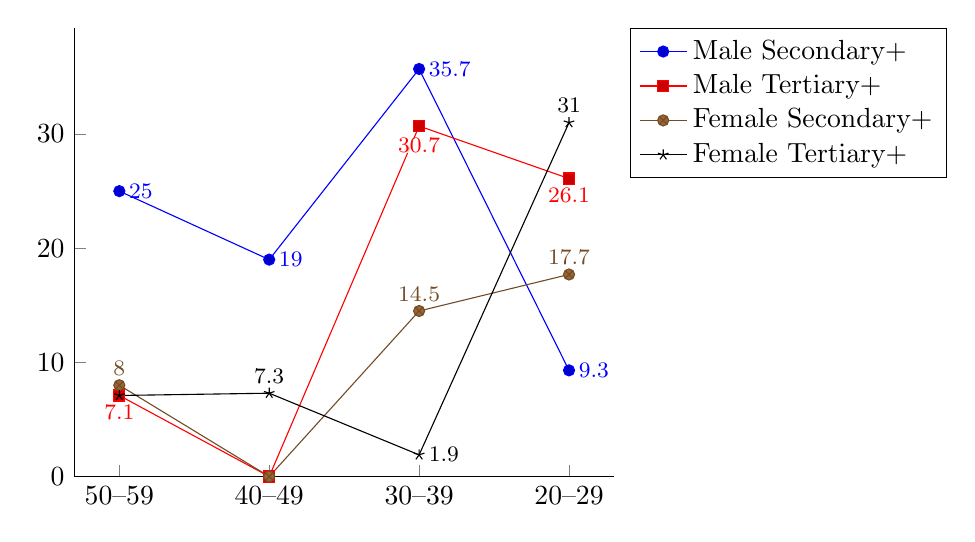
\begin{tikzpicture}
\begin{axis}[
        axis lines*=left,
        nodes near coords={\pgfmathfloatifflags{\pgfplotspointmeta}{0}{}{\pgfmathprintnumber{\pgfplotspointmeta}}}, % only print non-zero nodes
        every node near coord/.append style={font=\footnotesize},
        nodes near coords align=horizontal,
	xtick={0,1,2,3},
	xticklabels={50--59,40--49,30--39,20--29},
	x tick label style={},  
	ymin=0,
	legend style={
            cells={anchor=west},
            legend pos=outer north east,
        },
	]
\addplot+[sharp plot] coordinates { (0,25) (1,19) (2,35.7) (3,9.3)};
\addplot+[sharp plot,nodes near coords={}] coordinates { (0,7.1) (1,0) (2,30.7) (3,26.1)};
\node[below,font=\footnotesize,color=red] at (axis cs:0, 7.1) {7.1};
\node[below=1ex,font=\footnotesize,color=red,fill=white,inner sep=0pt,fill opacity=0.8,text opacity=1] at (axis cs:2, 30.7) {30.7};
\node[below,font=\footnotesize,color=red] at (axis cs:3, 26.1) {26.1};
\addplot+[sharp plot,nodes near coords align=vertical] coordinates { (0,8) (1,0) (2,14.5) (3,17.7)};
\addplot+[sharp plot,nodes near coords={}] coordinates { (0,7.1) (1,7.3) (2,1.9) (3,31)};
\node[above,font=\footnotesize] at (axis cs:1, 7.3) {7.3};
\node[right,font=\footnotesize,color=black] at (axis cs:2, 1.9) {1.9};
\node[above,font=\footnotesize] at (axis cs:3, 31) {31};
\legend{Male Secondary+, Male Tertiary+, Female Secondary+, Female Tertiary+}
\end{axis}
\end{tikzpicture}
\caption{Front diphthong use by age, gender and level of education\label{fig:4}}
\end{figure}
 


  Younger women generally and younger university graduates use noticeably more [ie] than their counterparts from older \isi{age} groups.  Young less educated men, in contrast, use more [e] than both older men of a similar \isi{education level} and others in their \isi{age} cohort in this sample.  Indeed, among 20--29 year old informants, there is no statistical difference between general male and female use (p > .50, χ\textsuperscript{2} = .24).  But in the same \isi{age} cohort, the tertiary educated are much more likely to diphthongize than the secondary educated (p < .001, χ\textsuperscript{2} = 11.48), whether male or female.  The data therefore suggest that use of the front dipthong may be emerging as a more acceptable feature of \isi{JE}, as reflected in the pattern for young women and the more highly educated.  This pattern is not apparent in the speech of young, less educated men who seem to produce more consistently the [e] that the data in previous sections would suggest is more prestigious.  One possible interpretation of the data here is that young men at \isi{JAMPRO} are more careful in their production of the prestige monophthong precisely because when they use the \isi{Creole} variant it is more likely to have negative associations than if used by women.  Young men in this context here are the group least presumed to be educated and least favoured in terms of how they present as prospective employees of \isi{JAMPRO}. 

 Among the older \isi{age cohorts} note that the data follow a more predictable pattern.  For the 30--39 year olds, men use more diphthongs than women and the secondary educated use more diphthongs than university graduates.  This would be expected, given the results so far for \isi{gender} and level of education that correlated fewer \isi{Creole} forms with women and the highly educated.  And for the 50--65 \isi{age} group, university graduates and secondary educated women showed similar use of the variants, with the latter approximating to the prestige monophthong variant much more than their male counterparts.  


\begin{table}
\begin{tabular}{l*{5}{r@{ }S}}
\lsptoprule
& \multicolumn{6}{c}{\textit{poor}  words} & \multicolumn{4}{c}{\textit{beer} words}\\
& \multicolumn{2}{c}{[ɔ]} &  \multicolumn{2}{c}{[u\textsuperscript{o}]}   & \multicolumn{2}{c}{[o]} & \multicolumn{2}{c}{[i\textsuperscript{e}r]} & \multicolumn{2}{c}{[er]} \\
\midrule
20--29 & 179 & (80.0\%) & 31 & (14.0\%) & 13 & (6.0\%) & 173 & (49.8\%)  & 175 & (50.2\%)\\
50--65 &  78 & (68.0\%) & 26 & (23.0\%) & 11 & (9.0\%) & 64  & (45.0\%)  &  77 & (55.0\%)\\\cmidrule(lr){2-7}\cmidrule(lr){8-11}
    &  \multicolumn{6}{c}{(p < .05, χ\textsuperscript{2} = 6.53)}  & \multicolumn{4}{c}{(p > .30, χ\textsuperscript{2} = .73)}\\
\lspbottomrule
\end{tabular}
\caption{Pre-rhotic mid-vowels by age\label{tab:3.50}}
\end{table}

When the pre-rhotic data are also considered, it is clear that the use of the [ie] diphthong is, as Alleyne noted some two decades ago (\citeyear[41]{Alleyne1980a}), quite widespread, particularly in younger speakers; and in these same speakers the \isi{back diphthong} is less produced in all environments.  So in this sample of \isi{JE} speech, \isi{front diphthong} use tends to be higher in those educated in the 1970s and 1980s than those educated in the 1940s and 1950s, whereas back \isi{diphthong use} is much less, particularly pre-rhotically where the [ɔ] is favoured.

\subsection{Group B variables and age}%3.4.2n

  There was no statistical difference between older and younger speakers for either \textit{butter} type words or for the use of palatalized stops in \textit{culture} type words.  Where there seems to be some difference in the \isi{age cohorts} is the -\textit{tion} ending, though the significance is above the critical level (p < .10, χ\textsuperscript{2} = 6.5).  What difference there is suggests that younger speakers are more likely to have a schwa in \textit{education} type words, while older speakers tend to produce the [ʃɔn] variant.  As with the other variables along the \isi{Creole}\slash English dimension, \isi{age} does not correlate here with more, or less, use of the \isi{Creole} form.


\begin{table}
\begin{tabular}{l*{4}{r@{ }S}}
\lsptoprule
& \multicolumn{2}{c}{[ʃan]} & \multicolumn{2}{c}{[ʃʌn]}&  \multicolumn{2}{c}{[ʃɔn]} &  \multicolumn{2}{c}{[ʃǝn]} \\
\midrule
20--29 & 52 & (22.0\%) & 118 & (50.5\%) & 35 & (15.0\%) & 29 & (12.5\%)\\
50--65 & 25 & (21.5\%) & 59  & (51.0\%) & 26 & (22.0\%) & 6  & (5.0\%)\\
\lspbottomrule
\end{tabular}
\caption{\textit{education} type words by age}
\label{tab:3.51}
\end{table}

Interestingly, while use of schwa did not index higher education, [ʃɔn] did, and has been reported elsewhere as more likely in speakers with longer exposure to schooling \citep[4]{Shields-Brodber1996}.  In addition [ʃɔn] is more a feature of the \isi{age} cohort educated during the \isi{colonial period} and presumably more exposed to British norms.  A more detailed picture of the use of the two variants is presented in \tabref{tab:3.52}.

\begin{table}
    \begin{tabular}{lrrrr}
	\lsptoprule
& \multicolumn{2}{c}{50--65} &  \multicolumn{2}{c}{20--29}\\
&                     Tertiary+ &  Secondary+   &  Tertiary+ & Secondary+\\\midrule
educa\textbf{[ʃɔn]}  &   14    &  11   &  25   & 10 \\
educa\textbf{[ʃǝn]}   &    4    &   2   &  6    & 23 \\
\lspbottomrule
\end{tabular}
\caption{\textit{education} type words by age and education}
\label{tab:3.52}
\end{table}

  Older speakers, regardless of level of education, tend to use the variants similarly – here more of the [ʃɔn] variant.  It is among young speakers that [ʃɔn] correlates with higher education and therefore a longer stay in the school system.  The highly educated young are therefore using the \isi{prestige norm} of older speakers, and it would therefore be difficult to argue for [ʃɔn] as an emerging variant in \isi{JE}.  Schwa use is highest in the young secondary educated speaker and, given the results for other sociolinguistic correlations, seems to be more peripheral in the speech community.

\begin{table}

\begin{tabular}{l*{4}{r@{ }S}}
\lsptoprule
 & \multicolumn{4}{c}{\textit{party} type words} & \multicolumn{4}{c}{\textit{forty} type words}\\
 & \multicolumn{2}{c}{[partɪ]} & \multicolumn{2}{c}{[pa:tɪ]}  & \multicolumn{2}{c}{[fɔ\textbf{rtI}]} & \multicolumn{2}{c}{[fɔ\textbf{:tI}]} \\
\midrule
20--29 & 54 & (58.0\%)  & 39 & (42.0\%) & 77 & (85.5\%) & 13 & (14.5\%)\\
50--65 & 13 & (41.0\%)  & 19 & (59.0\%) & 38 & (63.0\%) & 22 & (37.0\%)\\\cmidrule(lr){2-5}\cmidrule(lr){6-9}
  &     \multicolumn{4}{c}{(p < .10, χ\textsuperscript{2} = 2.91)}   &   \multicolumn{4}{c}{(p < .01, χ\textsuperscript{2} = 9.92)}\\\lspbottomrule
\end{tabular}
\caption{Rhoticity by age\label{tab:3.53}}
\end{table}

Younger speakers are more rhotic than older speakers, and in particular after the [ɔ] vowel.  

  \figref{fig:5} compares all \isi{age cohorts} with education in the production of \textit{forty} type words.  

\begin{figure}
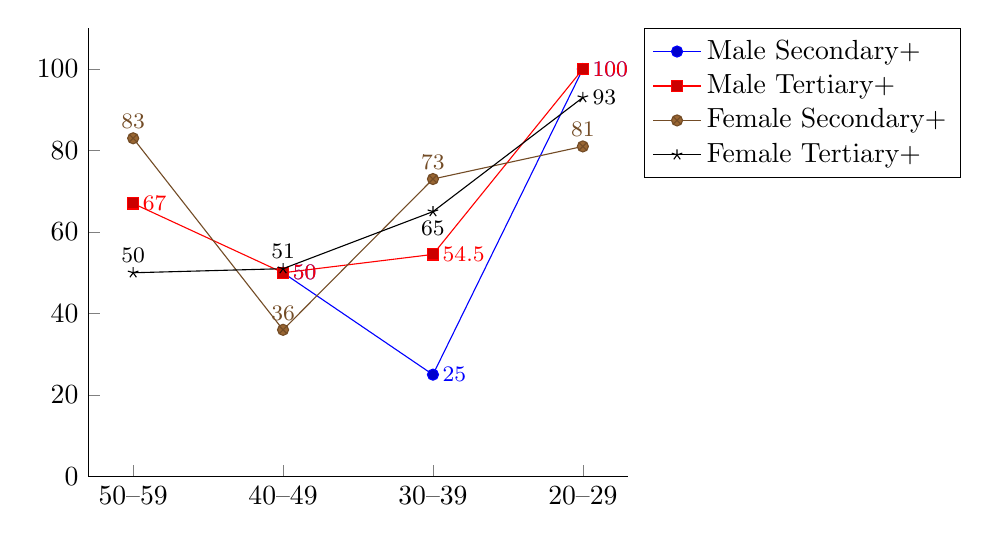
\begin{tikzpicture}
\begin{axis}[
        axis lines*=left,
        nodes near coords={\pgfmathfloatifflags{\pgfplotspointmeta}{0}{}{\pgfmathprintnumber{\pgfplotspointmeta}}}, % only print non-zero nodes
        every node near coord/.append style={font=\footnotesize},
        nodes near coords align=vertical,
	xtick={0,1,2,3},
	xticklabels={50--59,40--49,30--39,20--29},
	x tick label style={},  
	ymin=0,
	legend style={
            cells={anchor=west},
            legend pos=outer north east,
        },
	]
\addplot+[sharp plot, nodes near coords align=horizontal] coordinates { (1,50) (2,25) (3,100)};
\addplot+[sharp plot, nodes near coords align=horizontal] coordinates { (0,67) (1,50) (2,54.5) (3,100)};
\addplot+[sharp plot] coordinates { (0,83) (1,36) (2,73) (3,81)};
\addplot+[sharp plot,nodes near coords={}] coordinates { (0,50) (1,51) (2,65) (3,93)};
\node [font=\footnotesize,above] at (axis cs: 0,50) {50};
\node [font=\footnotesize,above] at (axis cs: 1,51) {51};
\node [font=\footnotesize,below] at (axis cs: 2,65) {65};
\node [font=\footnotesize,right] at (axis cs: 3,93) {93};
\legend{Male Secondary+, Male Tertiary+, Female Secondary+, Female Tertiary+}
\end{axis}
\end{tikzpicture}
\caption{Rhoticity after [ɔ] by age, gender and level of education.}
\label{fig:5}
\end{figure}

With the exception of the 4 primary educated informants, all speakers in this sample seem to be over time normalising \isi{rhoticity} after the back vowel [ɔ], a pattern which seemed to have been led by less educated females and more educated male speakers.  If we argue that the production of 50--65 year old female graduates, who cannot be characterized as either strictly rhotic or non-rhotic, reflected the instability of the sociolinguistic variable in terms of prestige, then there has been a conscious adoption of a rhotic \isi{prestige norm}.

When the patterns for the highest educated groups are analysed in terms of \isi{gender}, we see a divergence between men and women as it relates to \isi{rhoticity} generally.  Young educated men are less rhotic after [a], while following the rhotic pattern of others in the sample after the [ɔ] vowel.

           
\begin{figure}
\begin{tikzpicture}
\begin{axis}[
        axis lines*=left,
        nodes near coords={\pgfmathfloatifflags{\pgfplotspointmeta}{0}{}{\pgfmathprintnumber{\pgfplotspointmeta}}}, % only print non-zero nodes
        every node near coord/.append style={font=\footnotesize},
        nodes near coords align=vertical,
	xtick={0,1,2,3},
	xticklabels={50--59,40--49,30--39,20--29},
	x tick label style={},  
	ymin=0,
	legend style={
            cells={anchor=west},
            legend pos=outer north east,
        },
	]
\addplot+[sharp plot,nodes near coords={}] coordinates { (0,22.2) (1,25) (2,62.5) (3,71.4)};
\node [color=blue,font=\footnotesize,above] at (axis cs: 0,22.2) {22.2};
\node [color=blue,font=\footnotesize,below] at (axis cs: 1,25) {25};
\node [color=blue,fill=white,font=\footnotesize,below right=.75ex,inner sep=0pt, fill opacity=0.9, text opacity=1] at (axis cs: 2,62.5) {62.5};
\node [color=blue,font=\footnotesize,above] at (axis cs: 3,71.4) {71.4};
\addplot+[sharp plot,nodes near coords={}] coordinates { (0,50) (1,51) (2,65) (3,93)};
\node [color=red,font=\footnotesize,above] at (axis cs: 0,50) {50};
\node [color=red,font=\footnotesize,above] at (axis cs: 1,51) {51};
\node [color=red,font=\footnotesize,above] at (axis cs: 2,65) {65};
\node [color=red,font=\footnotesize,right] at (axis cs: 3,93) {93};
\addplot+[sharp plot] coordinates { (0,67) (1,87.5) (2,75) (3,40)};
\addplot+[sharp plot,nodes near coords={}] coordinates { (0,67) (1,50) (2,54.5) (3,100)};
\node [font=\footnotesize,below] at (axis cs: 1,50) {50};
\node [font=\footnotesize,below] at (axis cs: 2,54.5) {54.5};
\node [font=\footnotesize,above] at (axis cs: 3,100) {100};
\legend{\isi{rhoticity} [a] F, \isi{rhoticity} [ɔ] F, \isi{rhoticity} [a] M, \isi{rhoticity} [ɔ] M}
\end{axis}
\end{tikzpicture}
\caption{Post-vocalic rhoticity  after [a] and [ɔ] by age and gender.}
\label{fig:6}
\end{figure}


There is evidence, in the hypercorrect use of \isi{rhoticity}, the distancing from non-rhotic \isi{Creole} forms and the female pattern of \isi{rhoticity}, to suggest that \isi{rhoticity} is a normalised feature of \isi{SJE}.  The data for young men, who are less rhotic after [a], suggest two things however.  These young men are, as is found in other speech communities, producing more non-stan\-dard forms of the variable.  Moreover, as with the results for earlier correlations, \isi{rhoticity} after [a] is much more likely to be the site of sociolinguistic differentiation than after [ɔ].  Arguably, the sociolinguistic significance of having [ɔ] in the \isi{idiolect}, production of which may be more obvious in a rhotic phonetic environment, is one constraint on variation.  Alternatively, the [ɔ] variant is much more likely to have developed focussed norms of use, in this case a rhotic norm.  Masculinity may well be projected by “sounding tough” through the use of non-stan\-dard forms, to the extent that those forms are not also projecting something which carries greater stigma in the speech community, such as a lack of education or not being able to “speak properly” in a context of white-collar employment.  

The results for consonant cluster use suggest that younger and older speakers behave similarly.  Generally, both \isi{age cohorts} have higher rates of cluster production before vowels; and higher rates of -nt clusters than -st clusters.  The rates of production of clusters with morphological function are also very similar for both \isi{age cohorts} in this sample.  In all cases, there was no statistically significant difference between the \isi{age} groups. 

\section{Hypercorrection in the JAMPRO sample}\label{sec:3.5}

Hypercorrection in speech has been defined in two ways, both relating to an overproduction of particular forms in certain groups of speakers or in individuals.  \citet{Labov1972} described a pattern of variant use in the lower middle class New Yorker, such that “{\ldots}the lower-middle-class speakers go beyond the highest-status groups in their tendency to use the forms considered correct and appropriate for formal styles” (126).  In effect, their overproduction was in relation to the linguistic behaviour in other (higher status) classes of speakers and reflected a more consistent production of the prestige or standard variants of a variable such as [θ] or post-vocalic \isi{rhoticity}.  This type of \isi{quantitative hypercorrection} suggests more than merely which variants speakers in the community consider prestigious; it also reveals that these speakers hold an idea that certain (desirable) social characteristics are indexed by use of such forms, though their patterns of use betray some insecurity about how they do reflect place in the social structure \citep[138]{Silverstein2000}.   Quantitative \isi{hypercorrection} is also ``a synchronic indicator of linguistic change in progress" (\citealt[245]{Labov1968}), in particular the conscious adoption and spread of a perceived \isi{prestige form} as the standard, noted in the pattern of \isi{rhoticity} in the \isi{JAMPRO} sample.     

  The other type of \isi{hypercorrection} involves analogical error \citep[117]{Preston1989}.  Speakers aim to produce what they have identified as the prestige reflex of a form they have in their \isi{vernacular} and in the process ``replace" too many in the conversion.  \citet[66]{Trudgill1986} gives the example of [bʌʧr] \textit{butcher}, where speakers of Northern dialects of English have over-applied a rule that converts Northern [ʊ] (as in [lʊv] \textit{love}) to [ʌ] for prestigious \isi{RP}; and \citet[277]{Bobda2001} cites the example of the form [plaktɪs] \textit{practice} in an educated Kenyan speaker who is conscious of the stigma attached to [l {\textasciitilde} r] variation.  It is this latter type of \isi{qualitative hypercorrection} \citep{Janda1992} and aspects of its occurrence in speakers of \isi{JE} at \isi{JAMPRO} that I wish to discuss in this section.  

I should first point out that the features listed below are not the only instances of \isi{qualitative hypercorrection} in Jamaica.  For example, some Jamaican speakers produce such items as: 
\begin{enumerate}
\item\relax [stanʤarin] \textit{tangerine} or [sprɪkl] \textit{prickle.}  JC does not allow [st] clusters syllable initially, so that the JC cognates of English ‘stone’ or ‘stop’ become [tuon] or [tap].  In ‘tangerine’ therefore, by analogy, speakers insert the ``missing" onset [s].  
\item\relax [a:rva] \textit{harbour}, where [v] is used for cognate English items with either [b] or [v].  
\item\relax [amaʊn] \textit{among} or [laʊnz] \textit{lungs}, as [ʌŋ] typically occurs in JC in English cognates like \textit{down} or \textit{town}, the ``correct" ending [aʊn] is substituted.  
\item\relax [flɪtaz] \textit{fritters}, [talabrɛd] \textit{thoroughbred}, showing the [l {\textasciitilde} r] variation found in, for example, West African varieties of English \citep[135]{Holm1988}.  \citet[62]{Alleyne1980a} points out that this type of variation is somewhat archaic in Jamaica.
\end{enumerate}

These forms did not occur in my sample and are typically identified with more basilectal varieties of Jamaican speech \citep[40--47]{Cassidy1961}. Possible instances of \isi{hypercorrection} in my sample occurred with the following variables: 

\begin{enumerate}
\item  Word initial \isi{glottal fricative} /h/.  In my sample of speakers, eleven informants produced the hypercorrect pattern, as in [hoke] \textit{‘OK’} (F70) or [hebl] \textit{able} F74), but typically with single attestations.    

\item  The low back stressed vowel /ɔ/.  Forms in my sample like [rɪlɔks] \textit{relax} (M47), [sɔlǝrɪ] \textit{salary} (F53) and [bɔ:trum] \textit{bathroom} (F96) produced by\linebreak seven of my informants would suggest the kind of sensitivity to the feature discussed above and a belief that [ɔ] is the ``correct" reflex of [a].  

\item  The interdental fricatives /θ/ and /ð/.  In this data word initial voiced TH stopping seemed to be a general feature of \isi{JE}, but the same informants tended to avoid the voiceless alveolar variant.  I have heard hypercorrect use of the voiceless fricative in items in some Jamaican speech.  It was produced once in the \isi{JAMPRO} sample (F76 [θʌg] \textit{tug}).  Hypercorrect use of [ð] did not occur in my sample.

\item  The \isi{alveopalatal affricate}.  Two of my informants (F6, F10), on more than one occasion, produced the form [djunjʌ] \textit{junior}, a hypercorrect use of the palatalized stop; additionally, 6 other informants typically produced [dʌs] for the word \textit{just}, a possible avoidance of the \isi{affricate}.  It is, however, specifically the hypercorrect use of the palatalized stop that I wish to focus on in this section. 

\item  Post-vocalic \isi{rhoticity}.   Hypercorrect \isi{rhoticity} did occur in one informant (F16), who produced the forms [ɔrθɔrɪtɪ] \textit{authority} and [masarʤ] \textit{massage}.  In light of this, and the findings in this and earlier studies, for some \isi{JE} speakers ``correct" English is rhotic at least when word internally before a consonant.  No pronunciations such as [ʤǝmekʌr] \textit{Jamaica}, or [kjubʌr] \textit{Cuba} occurred in my sample.  

\item  The mid-\isi{front vowel} [e].   According to \citet[19]{Christie2003},
\begin{quote}[a]nother example of \isi{hypercorrection} is the pronunciation by some teachers and radio personalities in particular, of words such as \textit{fear} and \textit{here} with the same vowel sound as in \textit{fair} and \textit{hair}, in an unconscious effort to avoid \isi{Creole} pronunciations such as occurs in \textit{fies} `face'.\end{quote}
\end{enumerate}

In my own sample, this pronunciation also occurred, and was found in the speech of all but 4 of my sample of 82 speakers.  In addition, one informant (F57) produced the item [lez] \textit{liaise.}  This relatively new item in the \isi{JE} lexicon is bisyllabic.  This informant might have first converted this to a monosyllabic [liez] and then ``replaced" the diphthong with its monopthong reflex [e]. 

\tabref{tab:3.54} presents the number and types of informants who did produce the above hypercorrect forms.  

\begin{table}
\resizebox{\textwidth}{!}{\begin{tabular}{rrrrrrl}
\lsptoprule\relax
  [h] & [ɔ] & [θ] & [dj] & [r] & [e] &  \\\midrule
  11  & 7   &  1  &  2   &   1 &  78 & Number of informants (of 82)\\
  2   & 0   &  0  &  1   &   1 &  32 & Number with tertiary education (of 32)\\
  3   & 2   &  0  &  2   &   1 &  28 & Number with tertiary educated parents (of 28)\\
  9   & 6   &  1  &  2   &   1 &  64 & Number of women (of 67)  \\
  2   & 1   &  0  &  0   &   0 &  14 & Number of men (of 15)\\\lspbottomrule
\end{tabular}}
\caption{Qualitative hypercorrection in the JAMPRO sample\label{tab:3.54}}
\end{table}

A number of comments can be made about the data presented above.  The general pattern in this sample is for each informant to have one or two hypercorrect forms and to produce one or two instances of it in their texts.  The data on [e] is clearly different in type from the others, as it seems to be a normalized feature of these \isi{JE} speakers, used in variation with [ie] by nearly all informants (\citealt[xlvi]{Allsopp1996} suggests this is common in most varieties of Caribbean English).  And unlike hypercorrect [h] or [ɔ], for example, [e] in \textit{beer} type words is typical of the speech of the highly educated and of those from likely \isi{JE} speaking households.  In any case, to describe [fe:r] \textit{fear} as hypercorrect is to assume an external (metropolitan) model of English for the \isi{Jamaican speech community} and to stipulate that a vowel distinction between words such as \textit{fear} and \textit{fair} is necessarily standard.  

By inspection, hypercorrect forms occur more frequently in female speakers, though there is no statistical difference in the \isi{gender} distribution of [h] insertion.  I am unable to make any meaningful comment on this given the disproportionate number of women interviewed.  However, Patrick identifies \textit{speaky-spoky}, hypercorrect use of [h] and [ɔ], as perceived to be more associated with female speakers (\citeyear[45]{Patrick1997}).  If women are more aware of the prestige pattern in speech communities, and are more likely to promote what becomes the \isi{prestige form}, then it is perhaps not unexpected to find more \isi{hypercorrection} in their speech.  

The incidence of [h] insertion and hypercorrect [ɔ] is much higher than for the other features discussed.  In light of Patrick's analysis, it appears that the distribution of these two hypercorrect items in the Jamaican population is also much more general than the other five.  The historical record (see \sectref{sec:3.2}) would suggest that they have been aspects of the \isi{Jamaican speech community} from the earliest days.  Indeed, it is possible that their production is only a function of JC-to-\isi{JE} conversion diachronically, and they have become aspects of one variety of \isi{JE} selected by speakers from the speech community.  It is hypercorrect use of these two items that have emerged as \textit{the} register that indexes the locally pretentious speaker.  

Three of the informants produced more than one type of hypercorrect form.  Informant F6 used hypercorrect [h], [ɔ] and [dj] (as in the examples [hon] \textit{own}, [kɔ:r] \textit{car} and [djunjʌ] \textit{junior}).  She is young (under 30), secondary educated, and comes from a household headed by parents with relatively little education who in Jamaica are called ``higglers", roadside or market traders.  The other feature of note in her speech is a form like [juʤǝlɪ] \textit{usually}, with the \isi{affricate} more typical of \isi{Creole} varieties and stigmatized in \isi{JE}.  Informant F74 produced both of the hypercorrect forms described in \textit{speaky-spoky}, as in the examples [hebl] \textit{able} and [mɔ:kIt] \textit{market}.  She is over 50 years old, with a primary education and very likely to be a \isi{vernacular} \isi{Creole} speaker, given her general sociolinguistic profile.   For example, she typically used \isi{Creole} forms like [dis] \textit{just} and an almost invariant \isi{low vowel} /a/ in \textit{not} type words in her text.  The other informant, F16, produced hypercorrect \isi{rhoticity}.  She also tends to produce [ʃɔn] in \textit{education} type words.  Additionally, she does not TH stop, nor does she have "problems" with [h] or [ɔ].  She holds a Masters degree and comes from a household with educated parents (her father is a bursar, her mother an accounts clerk).

The distribution of hypercorrect forms in the sample suggests therefore that: 

\begin{itemize}
\item 
Feature 7 (described as ``hypercorrect" [e]) should not be included in this discussion which
 takes an \isi{endonormative approach} to what is to be termed standard or \isi{good English} in Jamaica.   

\item 
Hypercorrect [h] and [ɔ] are each most common in the sample and, arguably, across the  
continuum.  Indeed, when used together, they are common enough to be considered a stereotype of the comically ``elevated''\linebreak speaker in Jamaica. 
 
\item 
Hypercorrect [h], [ɔ], and possibly [θ], are less likely to be found here among highly 
educated \isi{JE} speakers.  These are infrequently occurring\linebreak items, at least in this sample, and therefore such associations must be impressionistic and very tentative.  However, most of the informants who did produce these forms were not tertiary educated or from households with educated parents.
 
\item 
The hypercorrect forms that I find in \isi{female speech} include more features and may suggest a greater sensitivity to a wider set of prestige variants than held by men.  The exaggerated forms in this sample are also more an aspect of \isi{female speech}.  This, of course, would not be unexpected.  Greater approximation to and awareness of prestige\slash standard forms is a well-doc\-u\-ment\-ed aspect of women in many speech communities.                  
\item 
The hypercorrect pattern on [dj] may be more a function of correcting a stigmatized form than the targeting of any \isi{prestige form} for conversion.
\end{itemize}

  This makes this last feature somewhat different from the other instances of \isi{hypercorrection} in which there is a focussed prestige target.  In this sample, as discussed in \sectref{sec:2.3} of this study, a number of speakers seem to avoid producing affricates.  Possible substitutes are stops [wɪt] \textit{which}, fricatives [ʒɛnǝrǝl] \textit{general} and the palatalized stop mentioned in this section.  Certainly the \isi{affricate} is the preferred variant of the highly educated in the particular lexical items in question; but in this social context, affricates also occur in \isi{Creole} and can be stigmatized in \isi{JE}, as in [trɛʤa] \textit{treasure}.  I argue that this explains the extent of the variation found in my sample for this feature.

\section{Constructing the acrolect, Standard Jamaican English}\label{sec:3.6}

The \isi{hypercorrection} I describe can be taken as one indication of what is perceived to be standard.  In addition, so can the prescriptions of the school curriculum and the variants selected by the most educated and those from backgrounds that predict more access to education.  The cumulative data suggest therefore the following is salient for speaking \isi{SJE} according to this analysis of certain phonological variables:

\begin{description}
\item[Consonants]
    \begin{enumerate}[label=\alph*)]
        \item[]
        \item the word initial \isi{glottal fricative} /h/ in words where /h/ has a phonemic contrast with its absence.
        \item the \isi{voiceless interdental fricative} in phonemic contrast with /t/. 
        \item the word initial \isi{velar stop} [k\textsuperscript{h}] before the \textbf{\textit{long}} \isi{low central vowel} [a\textbf{:}].
        \item post [ɔ] \isi{rhoticity}, specifically before [+ coronal] consonants in words like \textit{forty}.
        \item the word final phonological stop cluster [nt] before a following vowel. 
        \item the word final \isi{morphophonemic cluster} when a past tense marker.
    \end{enumerate}
\item[Vowels]
    \begin{enumerate}[resume*]
        \item[]
        \item the low back stressed vowel /ɔ/, in words like \textit{not} and \textit{possible}.  
        \item the mid tense vowel [o] as it occurs pre-consonantally, in items like \textit{goat}.
        \item the vowel [ɔ] in \textit{poor} type words. 
    \end{enumerate}
\end{description}    

For all other phonological features there was some interidiolectal variation, certainly correlated with \isi{gender} and \isi{age}, or the suggestion of developing norms of use in a context of such variation. 

When all the sociological data are considered for these 82 speakers, it is clear that social differentiation is typically located in features along the \isi{Creole}\slash English dimension.  Group A variables were included in this study precisely because they have been identified in the literature as having clear English and \isi{Creole} variants of variables.  In general the sociolinguistic correlations done for those features reveal that factors such as higher education, a more affluent background and being female are associated with a greater use of \isi{JE} variants.  Moreover, the results for some Group B correlations, specifically the low incidence of [a] in \textit{butter} and \textit{education} type words, are also an aspect of avoiding the \isi{Creole} variant and favouring the \isi{JE} [ʌ].  Indeed, the \isi{rhoticity} in much of the sample may, in part, be due to the coexistence with a non-rhotic JC.  

However, the pattern of variation for many of the variables studied here is more interesting, and less predictable, than merely the avoidance of \isi{Creole} forms.  Crucially, for many of the pairs of variables described here, the variant distribution in \tabref{tab:3.55} can be abstracted from the patterns that tend to occur in actual spoken \isi{JE}.

\begin{table}
\begin{tabular}{lcc}\lsptoprule
     &  \multicolumn{2}{c}{Typically used variant(s)}\\\cmidrule(lr){2-3}
                         &   Variable 1                          &  Variable 2\\\midrule
Interdental fricative   &    [d {\textasciitilde} ð]                       & [θ]  \\  
Mid-vowels              &    [ie {\textasciitilde} e]                      & [o]  \\
						&	 [ier {\textasciitilde} er]                    & [ɔr] \\
Palatalized velar stops &    [kja {\textasciitilde} k\textsuperscript{h}a] & [k\textsuperscript{h}a:]\\
Rhoticity               &  [ar {\textasciitilde} a:] & [ɔr]\\
\lspbottomrule
\end{tabular}
\caption{Asymmetrical pattern of variation on certain phonological variables\label{tab:3.55}}
\end{table}

Speakers in this sample of formal \isi{JE}, as used by generally well-educated informants, seem to assign asymmetrical sociolinguistic importance to variants of related variables.  One set of variants in their speech, those in the first column, is free to vary in the production of \isi{JE}.  The other set of variants is not, and speakers all seem to demonstrate some consensus in use of one – as shown in the second column.  In that respect, the \isi{architecture} of sociolinguistic variation in this sample of Jamaicans, distinguishes what I will call load-bearing or constructional structures, i.e. those necessary for producing \isi{JE}, from others that speakers show no imperative to either produce or avoid.  I use the term \isi{load-bearing} here because in constructing an edifice, certain elements are necessary for and essential to supporting the structure; others serve to give the structure its character.  I propose that the function of these \isi{load-bearing} variants is to identify the variety as \isi{JE}, and that without their presence in sufficient frequency, the speaker will not be interpreted by others as producing “good” English.  

\begin{table}
\resizebox{\textwidth}{!}{\begin{tabular}{lSrSrSSSr}
\lsptoprule
& \multicolumn{2}{c}{Education} & \multicolumn{2}{c}{Gender} & \multicolumn{2}{c}{Background} & \multicolumn{2}{c}{Age} \\
\multicolumn{1}{c}{Feature} & \multicolumn{1}{c}{Secondary} & \multicolumn{1}{c}{Tertiary} & \multicolumn{1}{c}{Male} & \multicolumn{1}{c}{Female} & \multicolumn{1}{c}{+Affluent} & \multicolumn{1}{c}{\textminus Affluent} & \multicolumn{1}{c}{20--29} & \multicolumn{1}{c}{50--65}\\
\midrule\relax
[θ] ‘thing’                     &  82.0\%  & 93\%   &  69.5\%   & 89\%      &  94.0\%     &  79.0\%  &   86.0\%     &  82\%\\{}
[ð] ‘then’                      &  44.0\%  & 51\%   &  34.0\%     &   48\%  &  40.0\%     &  52.0\%  &   40.0\%     &  47\%\\{}
[o] ‘boat’                      &  91.0\%  & 94\%   &  89.0\%     &   93\%  &  92.0\%     &  89.0\%  &   92.5\%   &  92\%\\{}
[e] ‘face’                      &  84.0\%  & 89\%   &  80.5\%   & 87\%      &  89.0\%     &  85.0\%  &   80.0\%   &  92\%\\{}
[ɔr] ‘poor’                     &  77.0\%  & 70\%   &  57.0\%     &   77\%  &  81.5\%     &  72.0\%    & 80.0\%   &  68\%\\{}
[er] ‘beer’                     &  49.0\%  & 60\%   &  46.0\%     &   56\%  &  63.0\%     &  47.0\%  &   50.0\%   &  55\%\\{}
[k\textsuperscript{h}a:] ‘calf’ &  72.0\%  & 91\%   &   76.5\% &  81\%      &  91.0\%     &  71.5\%  &   73.0\%   &  73\%\\{}
[k\textsuperscript{h}a] ‘cap’   &  39.0\%  & 48\%   & 41.0\%      & 44\%    &  43.0\%     & 42.0\%     & 46.0\%   &  44\%\\{}
[ɔr] ‘forty’                    &  73.0\%  & 61\%   & 62.0\%     &  67\%    &  65.0\%     & 69.0\%    &  80.0\%   &  68\%\\{}
[ar] ‘party’                    &  39.5\%  & 53\%   & 28.0\%      & 48\%    &  43.0\%     & 44.0\%     & 50.0\%   &  55\%\\\lspbottomrule
\end{tabular}}
\caption{Asymmetrical pattern of frequencies for certain phonological variables}
\label{tab:3.56}
\end{table}

  An illustration of this asymmetrical pattern of production can be seen in \tabref{tab:3.56}.  With the exception of the pre-consonantal mid vowels /e/ and /o/ which vary with diphthongs, for all social groups identified in this study there is a clear contrast between the rate of production of load-bearing variants (highlighted) and non load-bearing ones.  A further illustration of this difference is to be found in the productions of ‘can’t’ or ‘don’t’ in this sample.  Speakers produced forms such as [kjã:], [k\textsuperscript{h}ã:], [k\textsuperscript{h}a:nt] or [duõ], [dõ], [dont].  The first in each set is the one that seldom occurred in the data.  For the other two in each set, it is the presence of the variant [k\textsuperscript{h}] before the \isi{long vowel} or [o] that identifies the form as \isi{JE}, notwithstanding the presence of the JC nasal vowel or the \isi{cluster simplification} evident in the data presented in this chapter.  Moreover, I suggest that a speaker who carefully uses forms like [k\textsuperscript{h}at] \textit{cat} and [ðat] \textit{that} all the time, but produces [kja:t] \textit{cart} or [tɪn] \textit{thin} too often will not necessarily be seen as using \isi{JE}.

In the data collected here, the \isi{Creole} variants of the \isi{voiceless interdental fricative}, the mid back vowel before [r] and the \isi{velar stop} before a long [a:] for example are virtually non-existent in the educated speaker's formal language use.  Indeed, [uo] is seldom used by anyone in the sample, regardless of level of education.  In contrast, those same speakers use both the \isi{Creole} and \isi{JE} variants of the voiced interdental, the mid \isi{front vowel} and /ka/.  As such, some features in the Jamaican language continuum starkly distinguish JC use and \isi{JE} use – keeping the varieties discrete in a linguistic context where there is no sharp discontinuity between a functionally distinct JC and \isi{JE}. 

The logic of this proposition would predict a few things.  Firstly, \isi{qualitative hypercorrection} would be more likely to occur with load-bearing variables than with variables that are not load-bearing.  And indeed, the previous section point\-ed to the production of hypercorrect [θ] but not [ð] for example.  Secondly, because variant use is more focussed and more normalised for these load-bearing variables, social differentiation is going to be more starkly signalled by use of these variables, indexing, for example, by their absence the characteristics stereotypical of the monolingual JC speaker – little education, membership in the lower class and the like.  The mid-vowel /o/ is the exception in this sample, as all groups in this study consistently avoid use of the diphthong.  As such, and thirdly, \isi{group affiliation} among \isi{JE} speakers is therefore typically not going to be signalled by use of these load-bearing variables because they function to show primarily the variety one is speaking.  Acts of identity with a group, like \isi{gender} or \isi{age}, will more typically occur with the variables in column one – as was seen with male \isi{rhoticity} after [a] and younger speaker's greater use of [ie].

  \citet[271]{DevonishHarry2004} theorize that the relationship between JC and \isi{JE} phonology, for most Jamaicans, represents differential convergence, i.e. a type of linguistic convergence that facilitates speakers shifting between the two varieties while at the same time maintaining the distinctness necessary for the complementary socio-functional distribution of the two varieties.  The results here suggest that the mechanism for this involves the selection of one variable of a pair of related variables to attach stigma\slash prestige, while ignoring the other.  The polar lects are kept distinct for speakers through the salient variables, such as [θ], [ɔ], [h], [k\textsuperscript{h}a:], use of which signals \isi{JE} and formality for example.  This may well be a pattern of variation that distinguishes models of \isi{diglossia} involving discrete varieties from models of \isi{diglossia} involving varieties on a continuum like that in Jamaica.  The distinction discussed by Gair (cited in \citealt[272--273]{Paolillo1997}), between literary \isi{Sinhala} and formal spoken \isi{Sinhala} for example, points to differences between a written and a spoken functionally (H) variety.  Educated Jamaicans who write \isi{IAE}, as with educated Belizeans (\citealt[67--68]{Escure1997}), produce a formal spoken variety of English, \isi{SJE}, that displays distinct socio-phonetic characteristics from varieties of English in metropolitan speech communities.    

If one examines data from, for example, New York (\citealt[253]{Labov1966};\citeyear[100--104] {Labov1972}) or Louisiana \citep[254]{Dubois1998} for the \isi{interdental fricative}, this asymmetrical attention to variants does not seem to occur.  Certainly, the discussion in \citet[119]{Green2002} does show that in African \isi{American English} (AAE) word initial TH stopping occurs principally with the voiced interdental [ð].  AAE speakers do not really produce forms like ‘ting’ \textit{thing} or ‘tree’ \textit{three}, unless they are speakers of Gullah, but ‘dese’ \textit{these} and ‘dem’ \textit{them} are fairly commonplace.  However, the data from all these communities suggest that, typically, \isi{style shift} or the use of more \isi{formal speech} is signalled by an across the board reduction in TH stopping, not by reducing TH stopping on one variable and ignoring its counterpart.  Certainly, in \isi{careful speech} both voiced and voiceless TH stop variants seem to be minimized, as these studies do not suggest differences in patterning for the two related variables (\citealt[51]{Ervin-Tripp2001}; \citealt[94]{Labov2001}).  Indeed the two are often analysed as one variable in the published data.  And \citet[86--90]{Watt2000} shows that in Tyneside English, variants of the mid-vowels /e/ and /o/ are used with very similar frequencies to each other.  Arguably, the speech communities of New York, Louisiana and Newcastle operate within a different ideological framework, one in which there is one language – English – and “best speakerhood” (\citealt[286]{Silverstein1996}) is reflected in use of the Standard of that language.  Moreover, members of those communities believe there is one language, albeit with dialectal variation that can mark particular sets of speakers. 

In Jamaica, there are two related language varieties for speakers, Patwa and English, and best speakerhood is reflected in the bidialectal speaker.  Monolingual JC speakers are viewed negatively, as are monolingual English speakers.  Both are judged to be deficient in this context, the former “backward” and the latter “not a real Jamaican”.  These related but functionally distinct varieties are managed through structuring variation in such a way that some variables serve to identify the variety the speaker is using, given the linguistic overlap particularly at the phonolexical level.  

Generally, in my sample, the idea of what is JC seems to be focussed around certain features – voiceless TH stopping, [kja\textbf{:}], \isi{h-drop}, the \isi{back diphthong}.  In large part it is not using these features that defines the \isi{acrolect}, so that those with higher education, from more affluent backgrounds, and women’s language are characterized by very low frequencies or absence of these variants.  Additionally, \isi{JE} is also having a greater frequency of other variants – most importantly [ɔ], being rhotic and with t\slash d presence before following vowels.  

  A number of variants are in fact used all the time here by speakers, notwithstanding differences in social group – the \isi{voiceless interdental fricative}, [k\textsuperscript{h}a\textbf{:}], [nt] and past tense clusters before a following vowel.  In addition, the highly educated and/or those from backgrounds with educated parents tend to produce /h/ and mid-vowel monophthongs.  Interestingly, the data from younger speakers suggest that fewer categorically use [h] or [e], but more of them are rhotic, particularly after the back vowel. 

  Except for one informant in this sample, all speakers vary [ɔ] to some extent with [a]; but with the exception of the 4 with primary education, all informants produce low frequencies of the [a].   I suggest that \isi{rhoticity} after the back vowel and the palatalization of the \isi{velar stop} also serve to display possession of this vowel, in a context where not being “able” to distinguish [a] from [ɔ] is “one of the shibboleths of the speech community” \citep[272]{DevonishHarry2004}.  Rhotic articulation may distinguish the [ɔ] vowel in an item like [fa:ti] {\textasciitilde} [f ɔ:ti] \textit{forty} more clearly; and palatalization of the velar only before [a], again reinforces a distinction between [kat] {\textasciitilde} [kɔt] which may be either \textit{cat} or \textit{cot} in some speakers.  Moreover, \isi{JE} variants like [ʃɔn] in \textit{education} type words are also a function of avoiding [a].

The chapter to come explores the sociology of \isi{JAMPRO} as an organization and its allocation of staff to certain positions.  In doing so I wish to explore how these phonological features are distributed in the speech of \isi{JAMPRO} staff and, in particular, the speech of staff who are successful in the agency and get promoted into positions that reflect the public face of an agency of the Jamaican state.
